\documentclass[../notes.tex]{subfiles}

\pagestyle{main}
\renewcommand{\chaptermark}[1]{\markboth{\chaptername\ \thechapter\ (#1)}{}}

\begin{document}




\chapter{Nanomaterials and Intro to XRD}
\section{Nanomaterials}
\begin{itemize}
    \item \marginnote{1/3:}Contact Dr. Shevchenko at \href{mailto:eshevchenko@anl.gov}{eshevchenko@anl.gov} or \href{mailto:eshevchenko@uchicago.edu}{eshevchenko@uchicago.edu}.
    \item How to make nano.
    \begin{itemize}
        \item Top-down approach: Start with large, end with nano. Includes nanofabrication.
        \item Bottom-up approach: Solution-based approach.
        \begin{itemize}
            \item Scalable and cheap.
            \item Use an inorganic core with a coating.
        \end{itemize}
    \end{itemize}
    \item What nanoparticles look like.
    \begin{itemize}
        \item Differences in size, size distribution, shape, chemical composition, and structures.
        \item Different sizes (like atoms) and different shapes (like bacteria and viri).
    \end{itemize}
    \item Ancient nanoscience.
    \begin{itemize}
        \item The Lycurgus cup.
        \begin{itemize}
            \item A 4th-century Roman glass cage cup.
            \item Currently housed at the British Museum.
            \item Contains $\sim\SI{70}{\nano\meter}$ gold/silver nanoparticles.
            \item When front-lit, it appears green (light is scattered by larger NPs).
            \item When back-lit, it appears red (light is absorbed by NPs).
        \end{itemize}
        \item Hair dye.
        \begin{itemize}
            \item 2000 years ago from Greco-Roman times.
            \item Made of lead oxide (\ce{PbO}), slaked lime (\ce{Ca(OH)2}), and water (\ce{H2O}).
            \item The lead oxide combines with sulfur-rich peptides in the hair to make $\sim\SI{5}{\nano\meter}$ \ce{PbS} NPs.
        \end{itemize}
    \end{itemize}
    \item Applications of nanoparticles: Catalysis.
    \begin{itemize}
        \item Refining of petroleum (transformation of crude oil into gasoline, jet fuel, diesel oil, and fuel oils).
        \item Converter of automobile exhaust (reduction of nitrogen oxides [\ce{NO_x}] to \ce{N2} and \ce{O2}; oxidation of \ce{CO} to \ce{CO2}; oxidation of unburnt hydrocarbons to \ce{CO2 + H2O}).
        \item Hydrogenation of \ce{CO} (synthesis of fuels such as methane or methanol).
        \item Selective oxidation of hydrocarbons (synthetic fibers, plastics, and fine chemicals).
    \end{itemize}
    \item Methods of NP analysis: XRD, TEM, XANES, and XPS.
    \item Applications of nanoparticles: Displays.
    \begin{itemize}
        \item Semiconductor nanoparticles (e.g., solutions of \ce{CdSe} or \ce{InP} nanoparticles) emit different colors.
        \item Sony has announced that it will embed quantum dots in its latest flat-screen TV.
        \item QLEDs can be made out of \ce{CdSe}, \ce{CdS}, \ce{InP} coatings with silica, perovskite (\ce{CsPbX} where $\ce{X}=\ce{Cl},\ce{Br},\ce{I}$), and cesium lead halide salts.
    \end{itemize}
    \item Milestones in the synthesis of nanomaterials (a subjective and incomplete POV).
    \begin{itemize}
        \item Alexei Ekimov (late 1970s-1981, USSR): \ce{CuCl_x} and \ce{CdSe} in molten glass matrix (fluorescence, gradient colors).
        \item Alexander Afros (1982): Theoretical description of size effect.
        \item Louis Brus (1983, Bell Labs, US): \ce{CdS} in solution.
        \item Paul Alivisatos (UChicago) and Moungi Bawendi (MIT).
        \item Moungi Bawendi et al. (1993): Synthesis of monodisperse \ce{CdSe} nanoparticles --- a big one!
        \item Philippe Guyot-Sionnest (1996): Synthesis of core/shell nanoparticles.
        \item Paul Alivisatos (1997 and 2003): Synthesis of nanorods and tetrapods.
        \item Chris Murray and Shouheng Sun (2000): Synthesis of magnetic \ce{FePt} nanoparticles.
        \item Benoit Dubert (2007, France): Synthesis of \ce{CdSe} nanoplates (more stable, emission is polarized and directional).
        \item Maksym Kovalenko (2015): Synthesis of perovskites.
        \item Mostafe El-Sayed, Catherine Murphy, Peidong Yang, and Yunan Xia: Synthesis of \ce{Au} and \ce{Ag} nanoparticles.
    \end{itemize}
    \item Synthesis of nanoparticles.
    \begin{itemize}
        \item The 1993 Bawendi paper.
        \item The innovation was the synthesis of NPs in organic solvents, still widely used today.
    \end{itemize}
    \item LaMer model.
    \begin{itemize}
        \item Precursors under go nucleation, focusing, and "nano"-Ostwald ripening.
        \item Key idea: Separation of nucleation and growth in time.
    \end{itemize}
    \item Nanomaterials: State-of-the-art.
    \begin{itemize}
        \item The chemistry behind QD synthesis is rather simple compared to what is used by organic or coordination chemists, but the field sometimes lacks depth and chemical understanding.
        \item Indeed, only a fraction of reported results have been reproduced, and only a fraction of those have been understood and optimized.
        \item This is a big problem for AI/ML approaches.
        \item During the next 5-10 years, nanomaterials synthesis will progress mostly through systematic mechanistic studies.
    \end{itemize}
    \item Synthesis of nanocrystals without Ostwald Ripening.
    \begin{itemize}
        \item The nanocrystals form and grow during 0.1-1 minute after the start of the reaction.
        \item Annealing at high temperatures (\SIrange{250}{280}{\celsius}) is required to improve crystallinity.
        \item No change in particle size takes place upon the annealing.
        \item Tune particle size with nucleation, since growth proceeds until all monomer is consumed --- fast nucleation leads to many particles, which can only grow so large; slow nucleation leads to a few particles which can grow very large (conservation of end volume).
    \end{itemize}
    \item Synthesis with "artificial molecules."
    \begin{itemize}
        \item Rearrangement, addition, substitution, and elimination.
    \end{itemize}
    \item Hollow nanocrystals: Kirkendal Effect at Nanoscale.
    \begin{itemize}
        \item Uniform spherical cobalt nanocrystals can be synthesized by rapid pyrolysis of cobalt carbonyl in hot solvent.
        \item Hollow nanocrystals form after sulfidation reaction.
    \end{itemize}
    \item Kirkendal effect.
    \begin{figure}[h!]
        \centering
        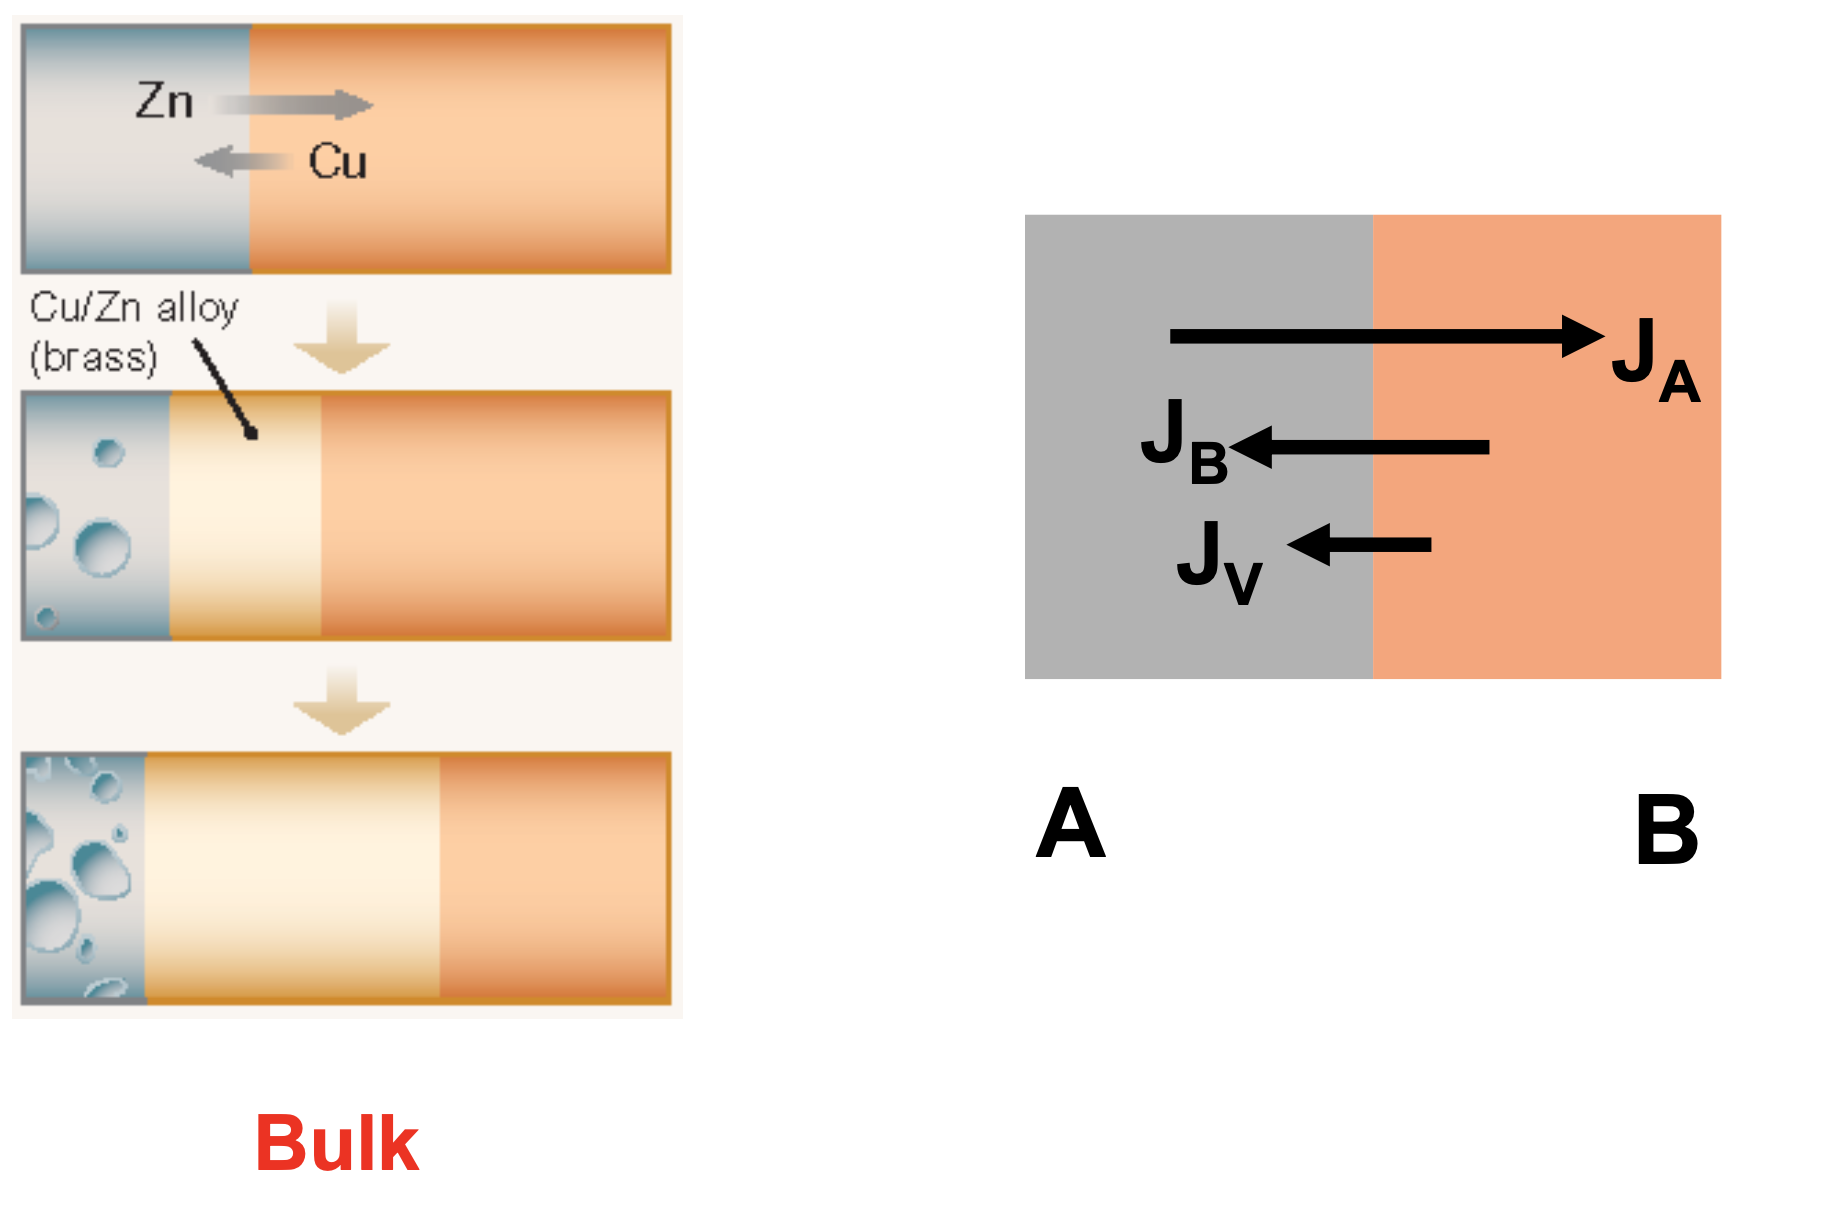
\includegraphics[width=0.43\linewidth]{KirkendalEffect.png}
        \caption{Kirkendal effect.}
        \label{fig:KirkendalEffect}
    \end{figure}
    \begin{itemize}
        \item Occurs when the diffusion rates of two species are different.
        \item When vacancies become supersaturated, they condense into voids in the fast diffusion species side.
        \item The Kirkendall voids result in weak bonding and lead to brittle fracture at the bonding interface.
    \end{itemize}
    \item Top-down approaches for the synthesis of \ce{MoS2}.
    \begin{figure}[h!]
        \centering
        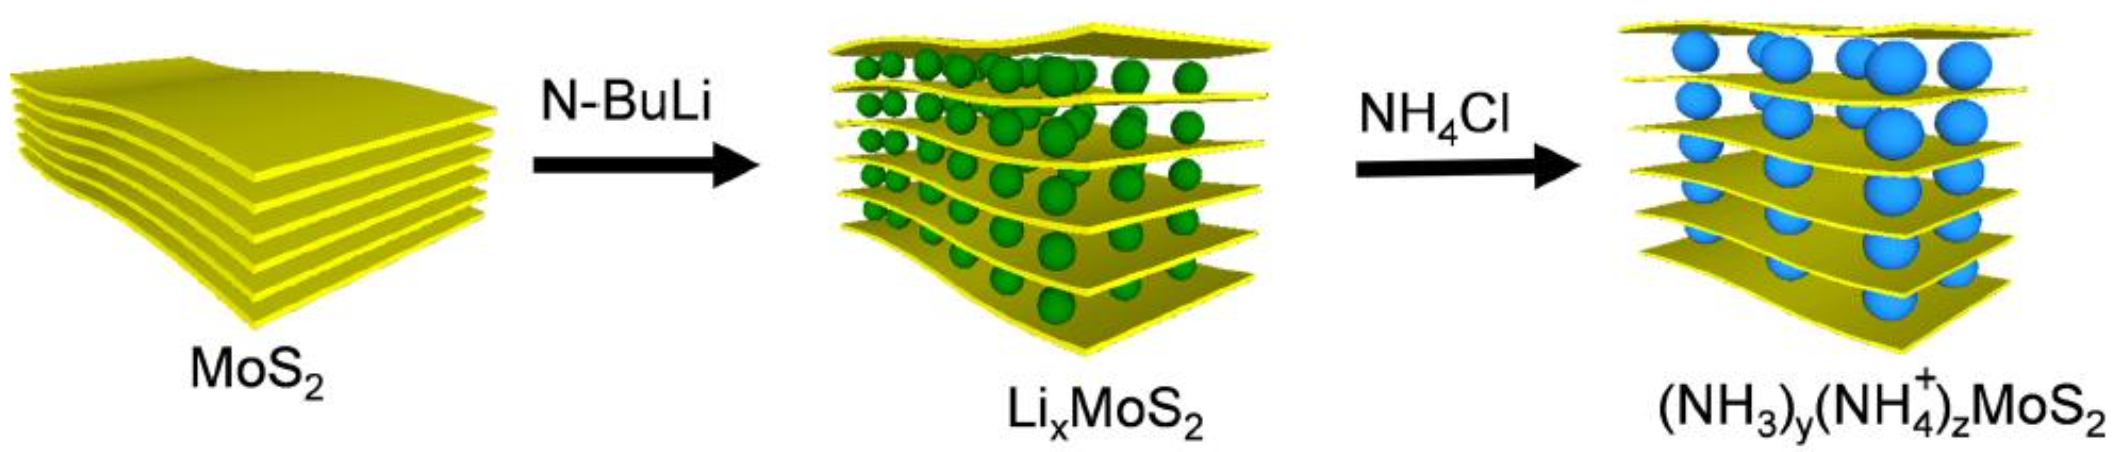
\includegraphics[width=0.6\linewidth]{topDownMoS2.png}
        \caption{Top-down synthesis of \ce{MoS2}.}
        \label{fig:topDownMoS2}
    \end{figure}
    \begin{itemize}
        \item This is the synthesis of interlayer expanded (IE) \ce{MoS2} through chemical intercalation of \ce{Li} and the following exchange with \ce{NH3} and \ce{NH4}.
        \item Each \ce{MoS2} layer is composed of an atomic layer of \ce{Mo} sandwiched between atomic layers of \ce{S} through strong ionic/covalent bonds. Weak van der Waals forces link individual \ce{MoS2} layers with an interlayer spacing of \SI{0.615}{\nano\meter}.
        \item Procedure.
        \begin{itemize}
            \item Electron-donating species, e.g., alkali metals, Lewis bases, and organolithium compounds can intercalate between layers.
            \item Alkali metals can after that be evaporated or react with water.
            \item \textbf{Exfoliation} with ultrasound (mechanical exfoliation).
        \end{itemize}
        \item Useful characterization methods: TEM, XRD, XPS.
    \end{itemize}
    \item \textbf{Exfoliation}: The complete separation of the layers of a material.
    \item Bottom-up approaches for the synthesis of \ce{MoS2}.
    \begin{itemize}
        \item Chemical synthesis of interlayer expanded (IE) \ce{MoS2}.
        \item Chemical Vapor Deposition (CVD).
    \end{itemize}
    \item MXene = 2D metal and surface chemistry.
    \begin{itemize}
        \item Applicatoins to supercapacitors, batteries, conductors, catalysts, and composites.
        \item Most made out of \ce{Ti3AlC2}.
    \end{itemize}
    \item MXenes: Solution processed 2D transition metal carbides and nitrides.
    \begin{itemize}
        \item Scanning electron microscopy (SEM) and HRTEM images shown.
        \item Etching and delamination phases.
    \end{itemize}
    \item MXenes: Variable termination groups.
    \begin{itemize}
        \item Ask in OH??
    \end{itemize}
    \item MXenes are solution processable 2D transition metal carbides and nitrides.
    \begin{itemize}
        \item Lists various experimentally synthesized structures.
    \end{itemize}
    \item What can and cannot be synthesized in solution?
    \begin{itemize}
        \item Current solution synthesis methodology can be applied to materials that crystallize below \SI{400}{\celsius}. Many materials that require higher temperatures to form, e.g., nitrides, carbides, \ce{GaAs}.
        \item Higher temperatures: Gas phase and solid state synthesis, as well as synthesis in molten salts.
    \end{itemize}
    \item Nanocrystals in molten salts.
    \begin{itemize}
        \item QDs are synthesized at high T in molten salts.
        \item There is typically a postpreparative treatment phase still in molten salts.
    \end{itemize}
    \item Nanoparticles as building blocks to make new materials.
    \begin{itemize}
        \item The idea behind nanoparticles is encapsulated by the synthesis of \ce{NaCl} from \ce{Na${}^\circ$} and \ce{Cl2${}^\circ$}: Two substances with certain properties combine to form a new material with very different properties.
        \item Assembly of atoms leads to new materials and new properties!
    \end{itemize}
    \item Self-assembly of nanoparticles.
    \begin{itemize}
        \item Can be multilayered (up to five).
    \end{itemize}
    \item Crystals of nanocrystals.
    \begin{itemize}
        \item Example: 3D crystals ($\sim\SI{30}{\micro\meter}$) have been assembled from \SI{3.3}{\nano\meter} \ce{CdSe} nanocrystals.
        \item Example: 3D crystals ($\sim\SI{10}{\micro\meter}$) have been assembled from \SI{6}{\nano\meter} \ce{CoPt3} nanocrystals.
        \item More conventional example: Crystals of quartz (made by atoms).
    \end{itemize}
    \item Binary nanoparticle superlattices.
    \begin{itemize}
        \item Natural opal vs. synthetic opals (very similar appearance and properties).
        \item Formation of binary superlattices depends on the ratio of nanoparticle radii ($\gamma$), the concentration of nanoparticles, the size distribution of nanoparticles, the nature of the capping ligand, and the substrate.
        \item Evaporating colloidal solutions of binary nanoparticle mixtures at \SI{45}{\celsius} leads to the formation of binary nanoparticle superlattices.
    \end{itemize}
    \item Periodic table of nanocrystals.
    \begin{itemize}
        \item Different types of unit cells listed.
        \item Examples include \ce{AlB2}, \ce{MgZn2}, \ce{Cu3Au}, \ce{Fe4C}, \ce{CaCu5}, and \ce{CaB6}.
    \end{itemize}
    \item Directing of self-assembly of nanocrystals.
    \begin{itemize}
        \item Various additives can be mixed in.
    \end{itemize}
    \item Metal organic frameworks (MOFs).
    \begin{itemize}
        \item MOFs (also called porous coordination polymers or PCPs) are two- or three-dimensional porous crystalline materials with infinite lattices synthesized from secondary building units (SBUs) --- metal cations, salts, or clusters --- and polydentate organic ligands with coordination type connections.
        \item Common SBUs pictured.
        \item From single-metal nodes to SBUs: More than 20,000 MOF structures have been reported so far.
        \item Characterization methods: TEM, SEM, XRD, XANES, XPS, and electron paramagnetic resonance (EPR).
    \end{itemize}
    \item Summary.
    \begin{itemize}
        \item Structural information (XRD, ED).
        \item Compositional information (XRD, ED, energy dispersive X-ray analysis [EDX], and X-ray fluorescence [XRF]).
        \item Size and morphology of materials (TEM, SEM, and XRD).
        \item Redox states of bulk and surface (XANES, XPS).
        \item Important variables: Quality of synthesized materials, stability of materials during processes, and structure-property correlations.
    \end{itemize}
\end{itemize}



\section{XRD Analysis}
\begin{itemize}
    \item \marginnote{1/5:}Applications of X-ray diffraction.
    \begin{itemize}
        \item Geology, environmental science, material science, engineering, biology.
        \item Originally developed for analysis of minerals.
    \end{itemize}
    \item What you can do with it.
    \begin{itemize}
        \item Characterization of crystalline materials (structure, unit cell, etc.).
        \item Identification of unknown/new crystalline materials (e.g., minerals, meteorites, etc.; rarely something on Earth since all of that has been extensively studied).
        \item Evaluation of sample purity.
    \end{itemize}
    \item XRD sample types: Can be used to characterize powders and thin films.
    \item Popular because\dots
    \begin{itemize}
        \item It's relatively inexpensive.
        \begin{itemize}
            \item There are benchtop instruments as well as larger ones.
        \end{itemize}
        \item It's relatively universal.
        \begin{itemize}
            \item Standardized procedures.
        \end{itemize}
        \item It's nondestructive.
    \end{itemize}
    \item Building blocks of X-ray diffractometers.
    \begin{itemize}
        \item \textbf{X-ray tube}, sample, \textbf{backstop}, \textbf{goniometer}, \textbf{collimator}, \textbf{filter/monochromator}, \textbf{detector}, \textbf{shutter}, and \textbf{safety interlock}.
        \item Basic definitions now; more on each of these devices later.
    \end{itemize}
    \item \textbf{X-ray tube}: The shield around the X-ray tube.
    \item \textbf{Backstop}: The device located behind the sample that absorbs non-diffracted X-rays. \emph{Also known as} \textbf{beam trap}.
    \item \textbf{Goniometer}: The mechanism that allows you to adjust the position of the sample relative to the incident X-ray beam.
    \item \textbf{Collimator}: The device that narrows the beam of X-rays.
    \item \textbf{Filter/monochromator}: The instrument that diffracts X-rays from a crystal to produce a beam comprising a narrow range of wavelengths.
    \item \textbf{Detector}: The device that measures diffraction patterns or energy spectra generated as a result of the interaction of X-rays with the sample.
    \item \textbf{Shutter}: The safety device (made of tungsten, tantalum, lead, etc.) inserted into the beam pass to stop all X-rays.
    \item \textbf{Safety interlock}: The device that stops the generation of X-rays when access to the interior part of the diffractometer is possible.
    \item How are X-rays generated?
    \begin{itemize}
        \item Originally with a \textbf{Crookes tube}.
    \end{itemize}
    \item \textbf{Crookes tube}: A type of discharge tube that facilitated the initial discovery of X-rays.
    \begin{itemize}
        \item History.
        \begin{itemize}
            \item Invented between 1869-1875 by William Crookes, who also discovered thallium.
            \item Wilhelm Roentgen was responsible for the initial discover of X-rays --- using a Crookes tube --- in 1895.
        \end{itemize}
        \item Design.
        \begin{itemize}
            \item Cold cathode vacuum tubes (no heated filament; these emit more electrons than can be supplied by thermionic emission alone).
            \item Relies on electron emission induced by an electrostatic field or secondary electron emission.
            \item Requires a small amount of gas (air) in them to function (\SIrange{e-6}{5e-8}{\atmosphere}).
            \item High voltage is applied to the tube.
            \item Electric current causes the ionization of gas molecules: Electrons "knock off" electrons from other gas molecules forming positive ions an negative electrons (negative ions are also formed as a result of electron interactions with neutral gas molecules).
            \item High velocity electrons hit the anode (metal) that creates the X-rays.
        \end{itemize}
    \end{itemize}
    \item The first images obtained using X-rays.
    \begin{itemize}
        \item The first medical X-ray was by R\"{o}ntgen (alternate spelling of Roentgen) of his wife in 1885.
        \begin{itemize}
            \item It led Roentgen to win the first ever Nobel in physics in 1901.
        \end{itemize}
        \item People started making X-rays of their bones just for fun --- like taking selfies --- without realizing the harm of X-rays.
        \item Some doctors notice improvement in cancer patients after X-ray exposure.
    \end{itemize}
    \item X-rays were discovered accidentally.
    \begin{itemize}
        \item A Crookes tube was wrapped in black cardboard to block the visible light.
        \item A fluorescent screen painted with phosphor barium platinocyanide (\ce{Ba[Pt(CN)4]}) was $\sim\SI{1}{\meter}$ away.
        \item When the tube was activated, the screen glowed green.
    \end{itemize}
    \item Limitations of Crookes tubes.
    \begin{itemize}
        \item X-rays originate from a rather large area. Thus, the resulting X-ray images lack contrast.
        \item Low intensity of X-rays; necessitates long exposures of the object.
    \end{itemize}
    \item Thus, Willian Coolidge develops the Coolidge tube in 1913.
    \begin{itemize}
        \item This is a hot cathode tube.
        \item It works with a much higher vacuum ($\sim\SI{e-9}{\atmosphere}$).
        \item Irving Langmuir designs an "extreme vacuum" with a new pump design (the Langmuir pump).
        \item This enabled generation of an electron current using a hot thermionic filament as the cathode.
        \item Other improvements.
        \begin{itemize}
            \item Replaced \ce{Pt} target with \ce{W}.
            \item \ce{Mo} shield to focus the X-rays.
        \end{itemize}
        \item These improvements led to\dots
        \begin{itemize}
            \item An X-ray source of remarkable brilliance and reliability;
            \item Control over intensity and hence penetrating power.
        \end{itemize}
        \item Since then, basically nothing has changed, though we did start using rotating anodes (see below).
    \end{itemize}
    \item Working principle of the X-ray tube.
    \begin{figure}[h!]
        \centering
        \begin{subfigure}[b]{0.4\linewidth}
            \centering
            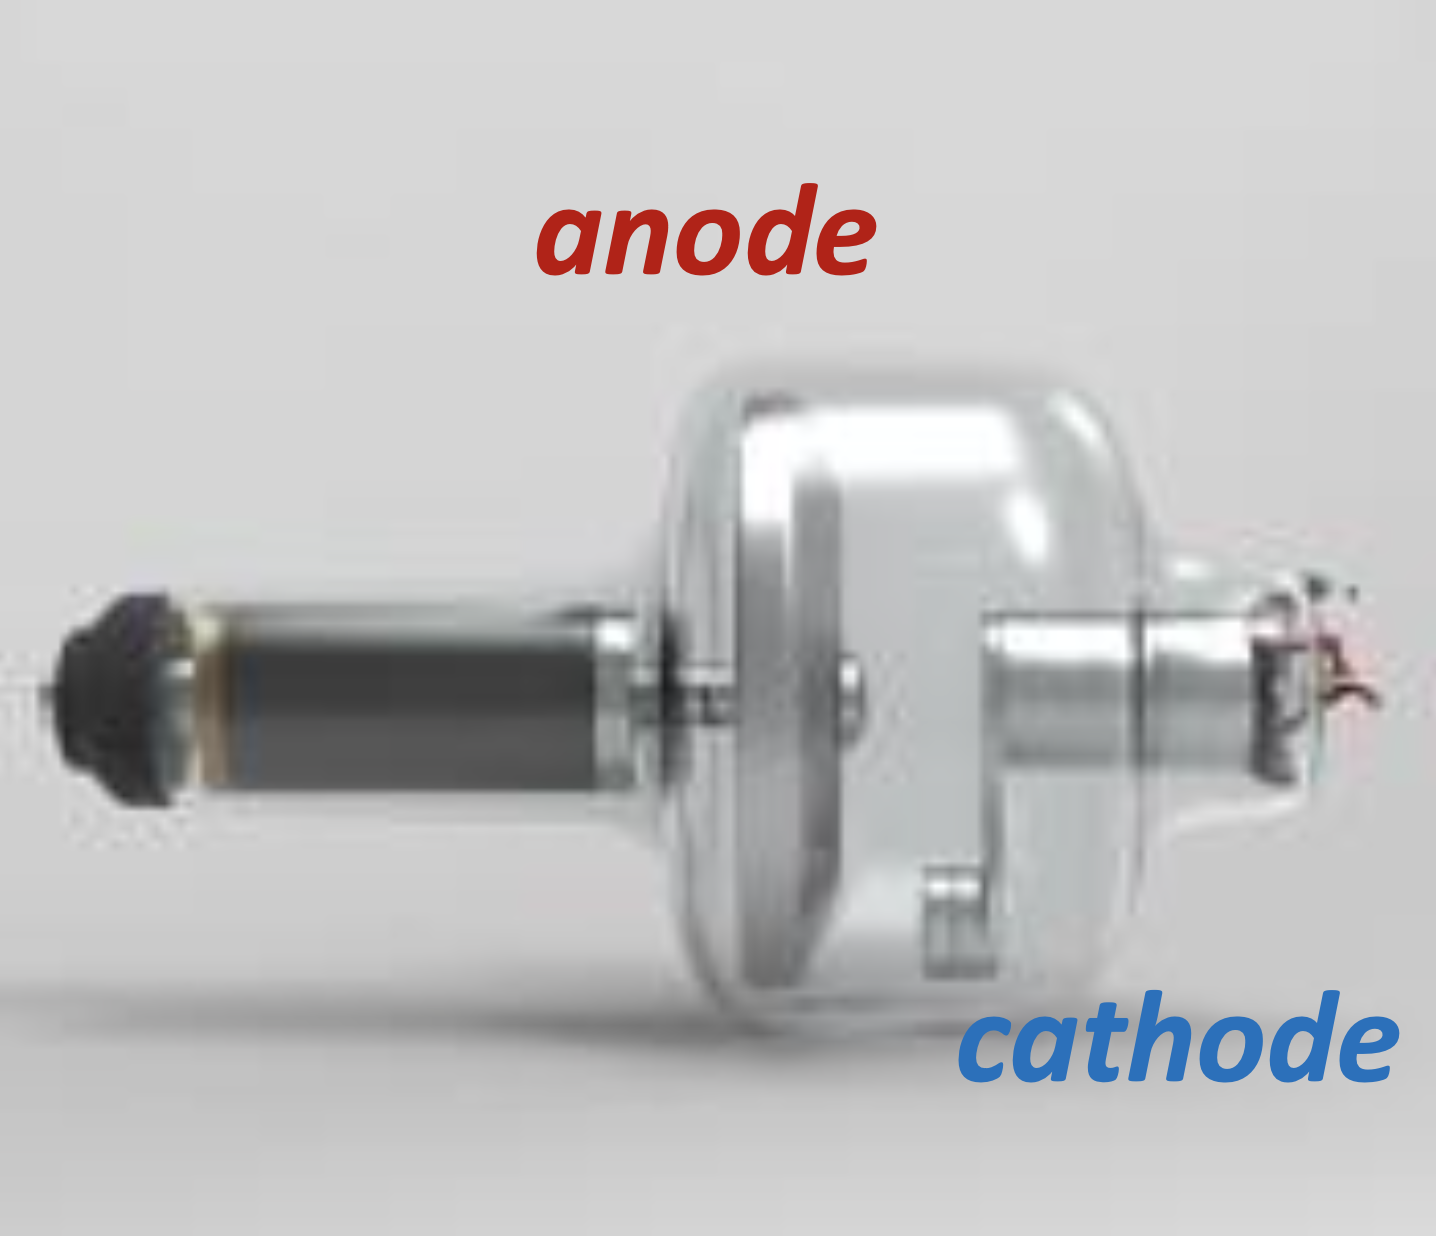
\includegraphics[width=0.8\linewidth]{xrayTubea.png}
            \caption{Overall design.}
            \label{fig:xrayTubea}
        \end{subfigure}
        \begin{subfigure}[b]{0.4\linewidth}
            \centering
            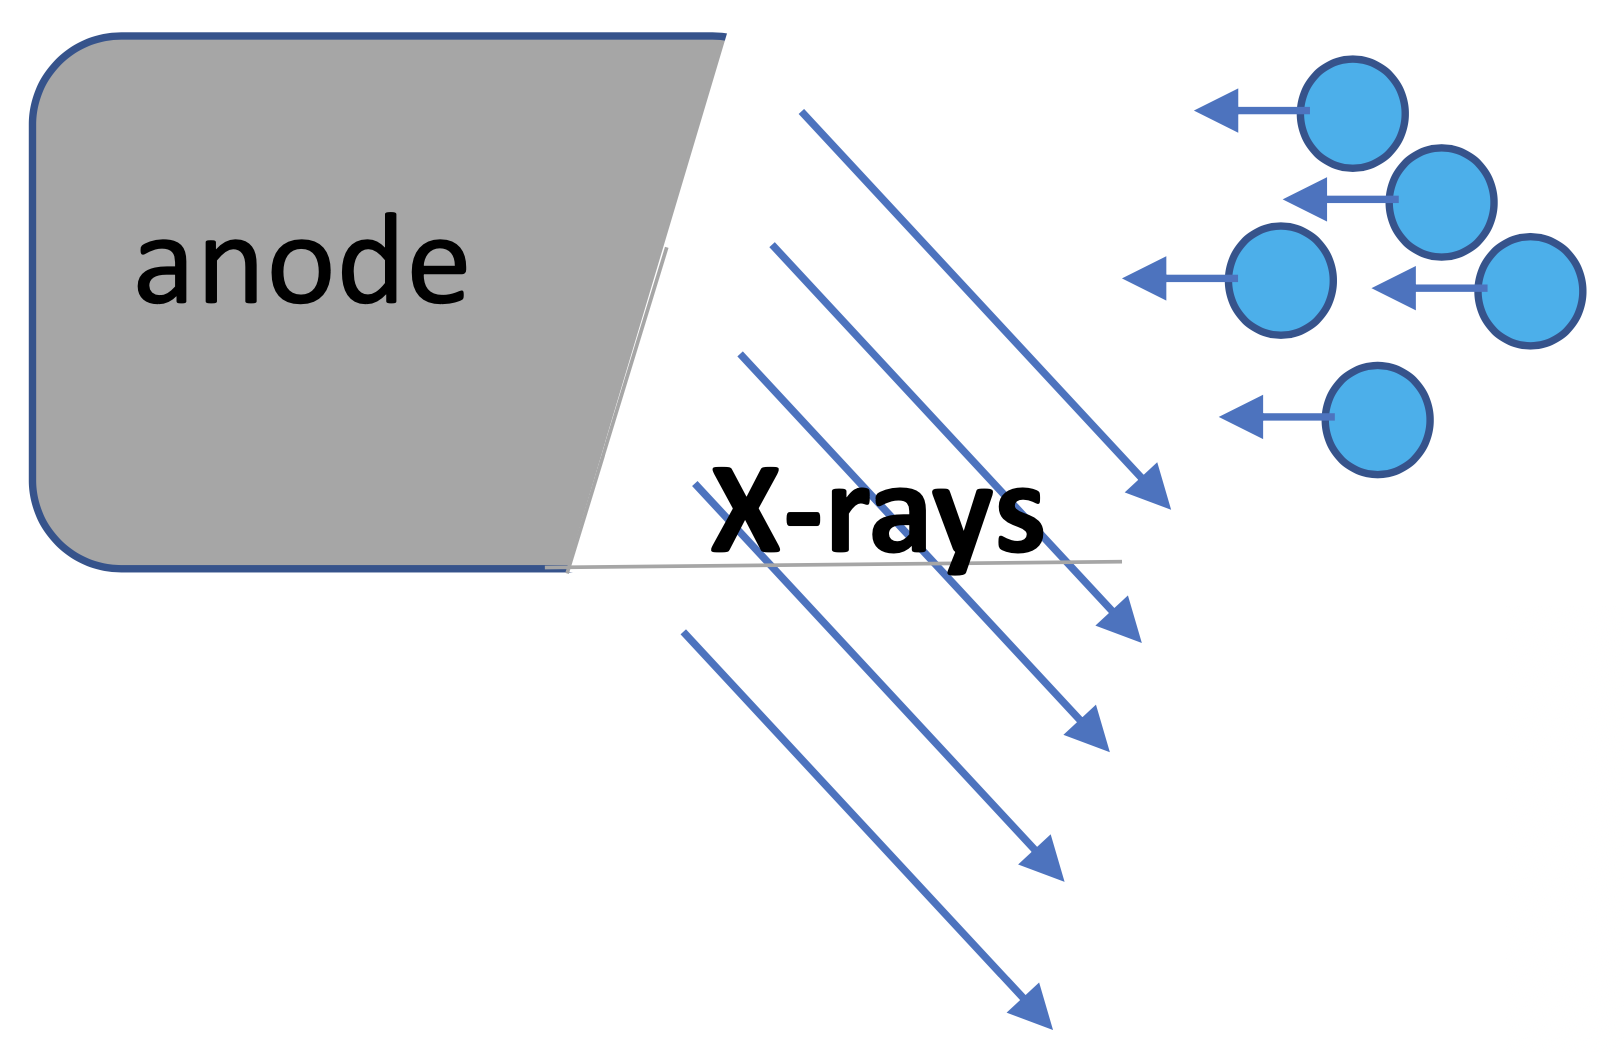
\includegraphics[width=0.8\linewidth]{xrayTubeb.png}
            \caption{Electrons to X-rays.}
            \label{fig:xrayTubeb}
        \end{subfigure}
        \caption{X-ray tube design.}
        \label{fig:xrayTube}
    \end{figure}
    \begin{itemize}
        \item The \textbf{cathode} heats up and induces thermionic emission of a cloud of electrons.
        \item The \textbf{anode} attracts the electrons across the vacuum tube.
        \item The anode converts the energy of incident electrons into X-rays, dissipating heat as a byproduct.
        \item You rotate the anode very fast (up to \SI{10000}{\revolutionsperminute}) to prevent it from overheating (can get up to \SI{2000}{\celsius}). This is why you often have a cooling system in high-power X-rays.
        \item The anode is a beveled disk (shaped to focus the X-rays).
        \item Most X-ray tubes have an \textbf{anode angle} of \SIrange{12}{15}{\degree}.
        \begin{itemize}
            \item A smaller angle results in a smaller effective \textbf{focal spot}.
        \end{itemize}
    \end{itemize}
    \item \textbf{Cathode}: The negatively charged filament.
    \item \textbf{Anode}: The positively charged disk. \emph{Also known as} \textbf{anticathode}.
    \item \textbf{Anode angle}: The angle between the vertical and the target surface.
    \item \textbf{Focal spot}: The surface area on the anode over which X-rays are produced.
    \begin{figure}[h!]
        \centering
        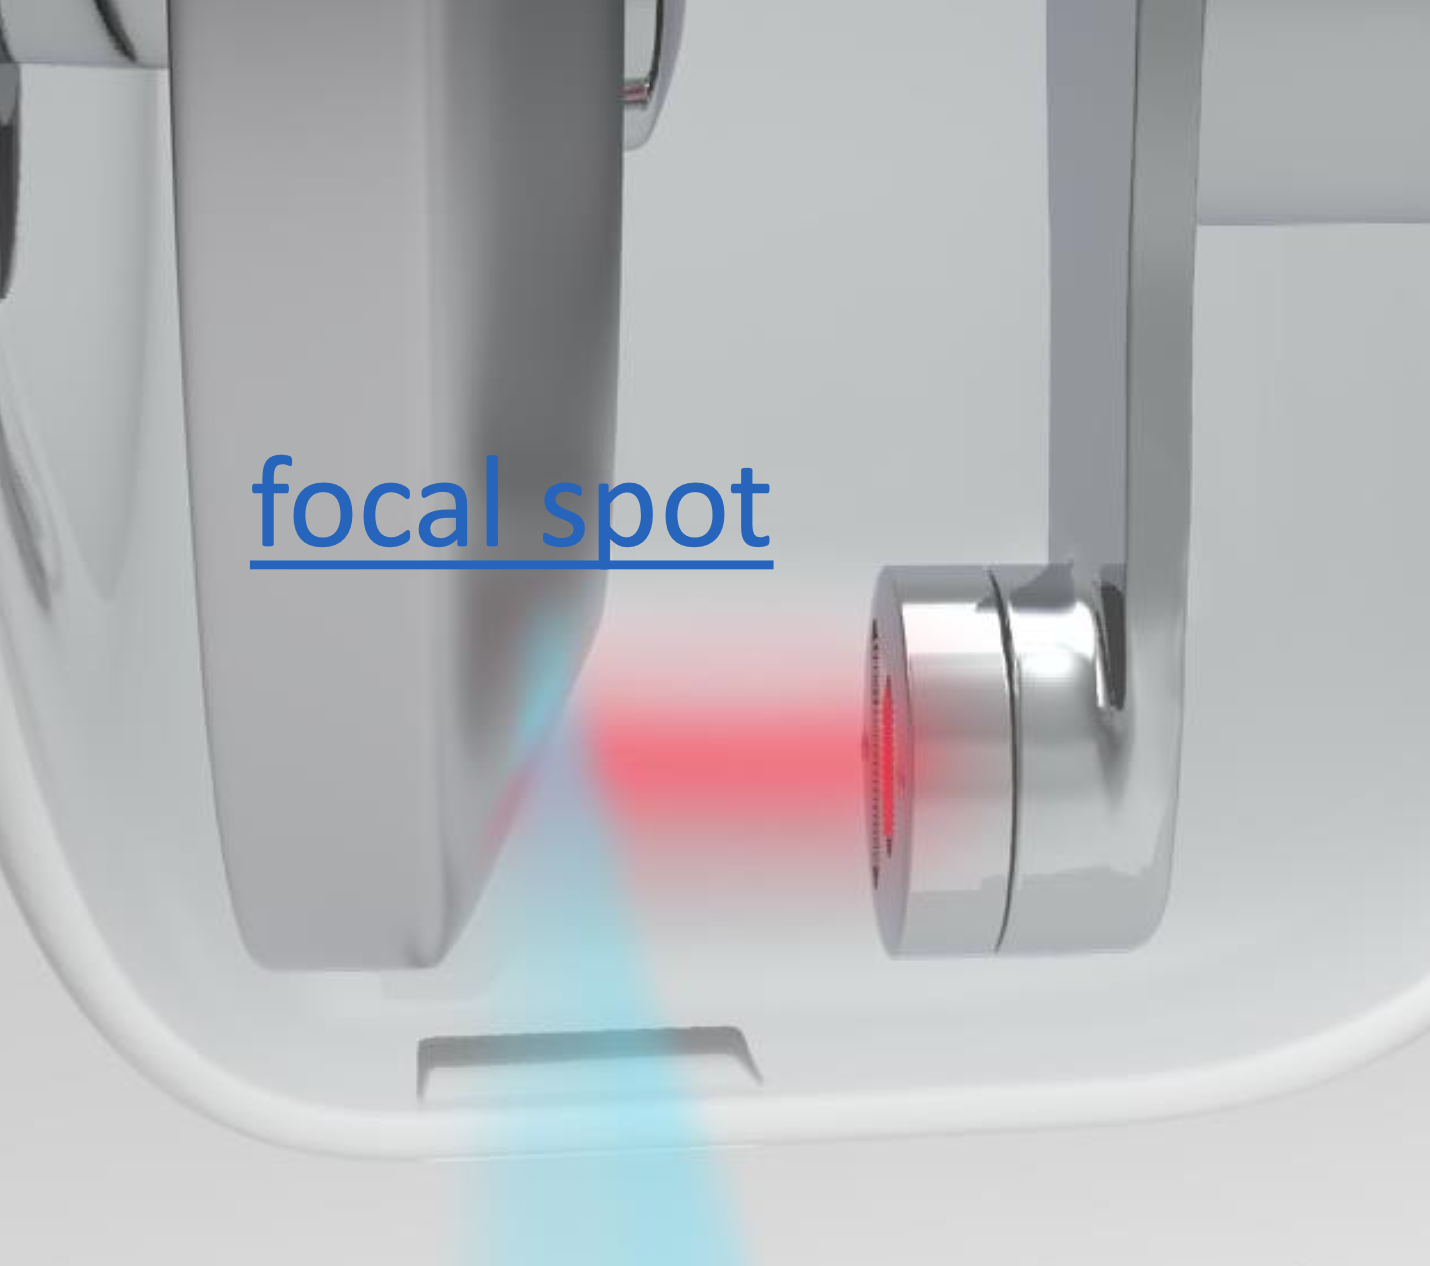
\includegraphics[width=0.3\linewidth]{focalSpot.png}
        \caption{Anode focal spot.}
        \label{fig:focalSpot}
    \end{figure}
    \begin{itemize}
        \item Naturally, increasing the angle will allow the electrons to spread out over more area.
    \end{itemize}
    \item Design of the X-ray tube.
    \begin{figure}[h!]
        \centering
        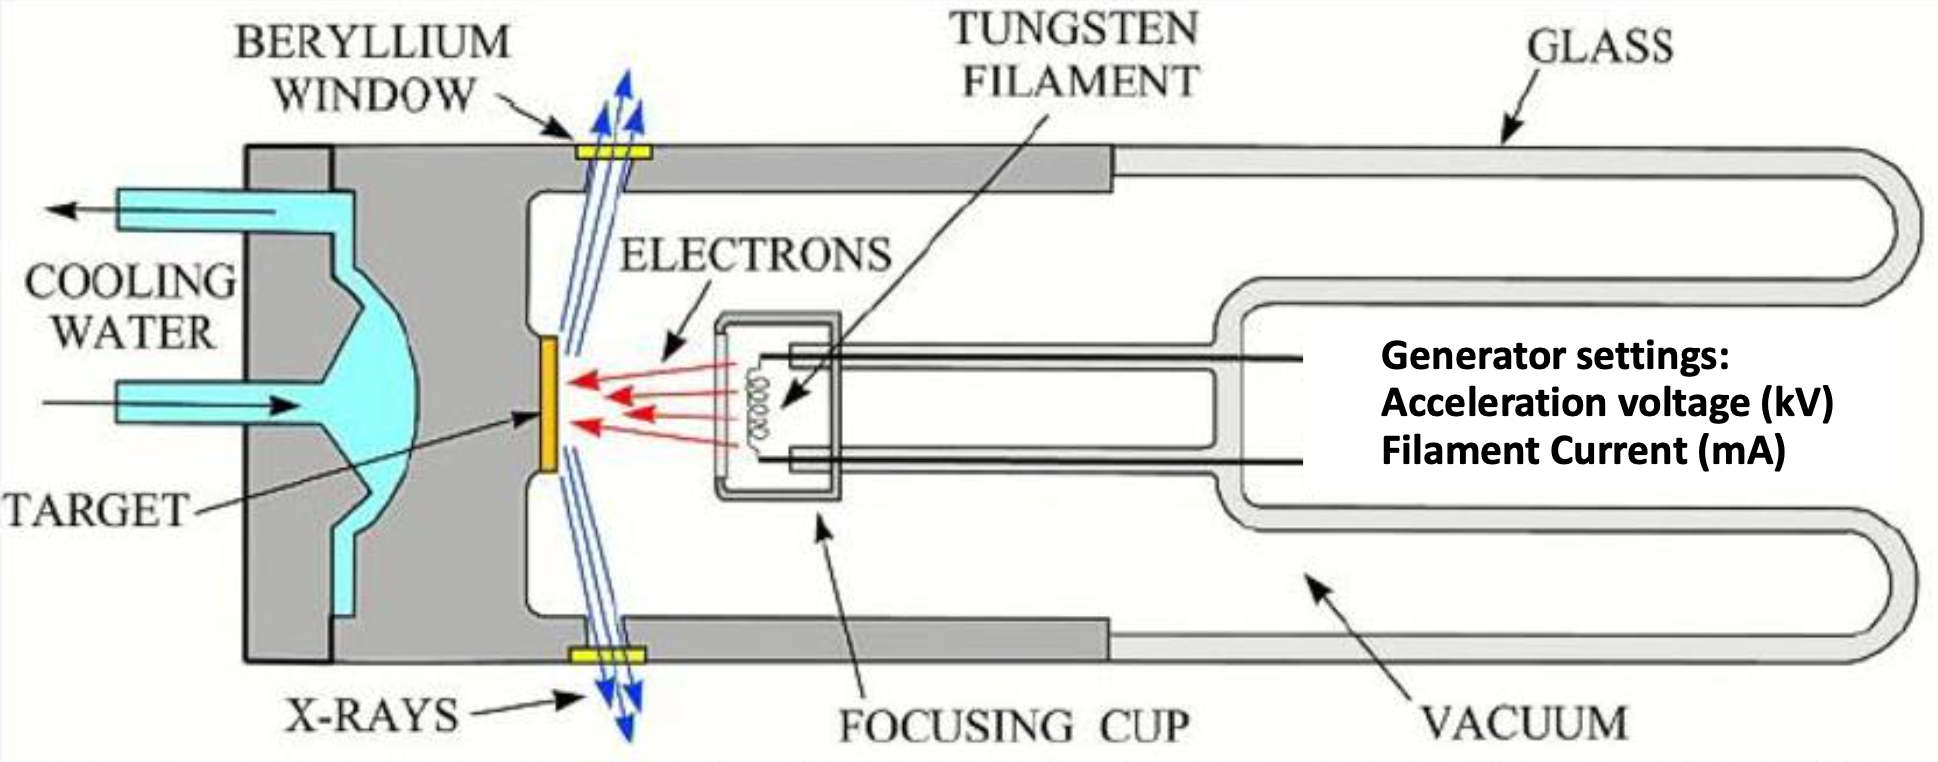
\includegraphics[width=0.7\linewidth]{xrayTubeSchematic.png}
        \caption{Schematic cross section of an X-ray tube.}
        \label{fig:xrayTubeSchematic}
    \end{figure}
    \begin{itemize}
        \item Beryllium is used as a window because it doesn't absorb X-rays, even though it's toxic.
        \item Beryllium has low X-ray absorbance because it is a very small atom. In technical terms, it has low \textbf{contact} (see below).
    \end{itemize}
    \item A few practical comments on the anode (filament).
    \begin{itemize}
        \item Lifetime of $\sim\SI{2000}{\hour}$ (at $\sim\SI{50}{\kilo\volt}$ and $\SI{200}{\milli\ampere}$).
        \item Reducing the tube current to \SI{100}{\milli\ampere} increases the lifetime by 50\%.
        \begin{itemize}
            \item Are there drawbacks to doing this?? Less intense X-rays, perhaps? Ask in OH.
        \end{itemize}
        \item The lifetime of the cathode depends on the number of times the X-ray source is turned on and off.
        \begin{itemize}
            \item Turning the XRD system on and off stresses the filament as well as other components.
            \item It is better to keep the XRD system on and in stand-by settings (power of $\sim\SI{20}{\kilo\volt}$ and current of $\sim\SI{10}{\milli\ampere}$).
        \end{itemize}
    \end{itemize}
    \item The spectrum of X-rays generated in an X-ray tube.
    \begin{figure}[H]
        \centering
        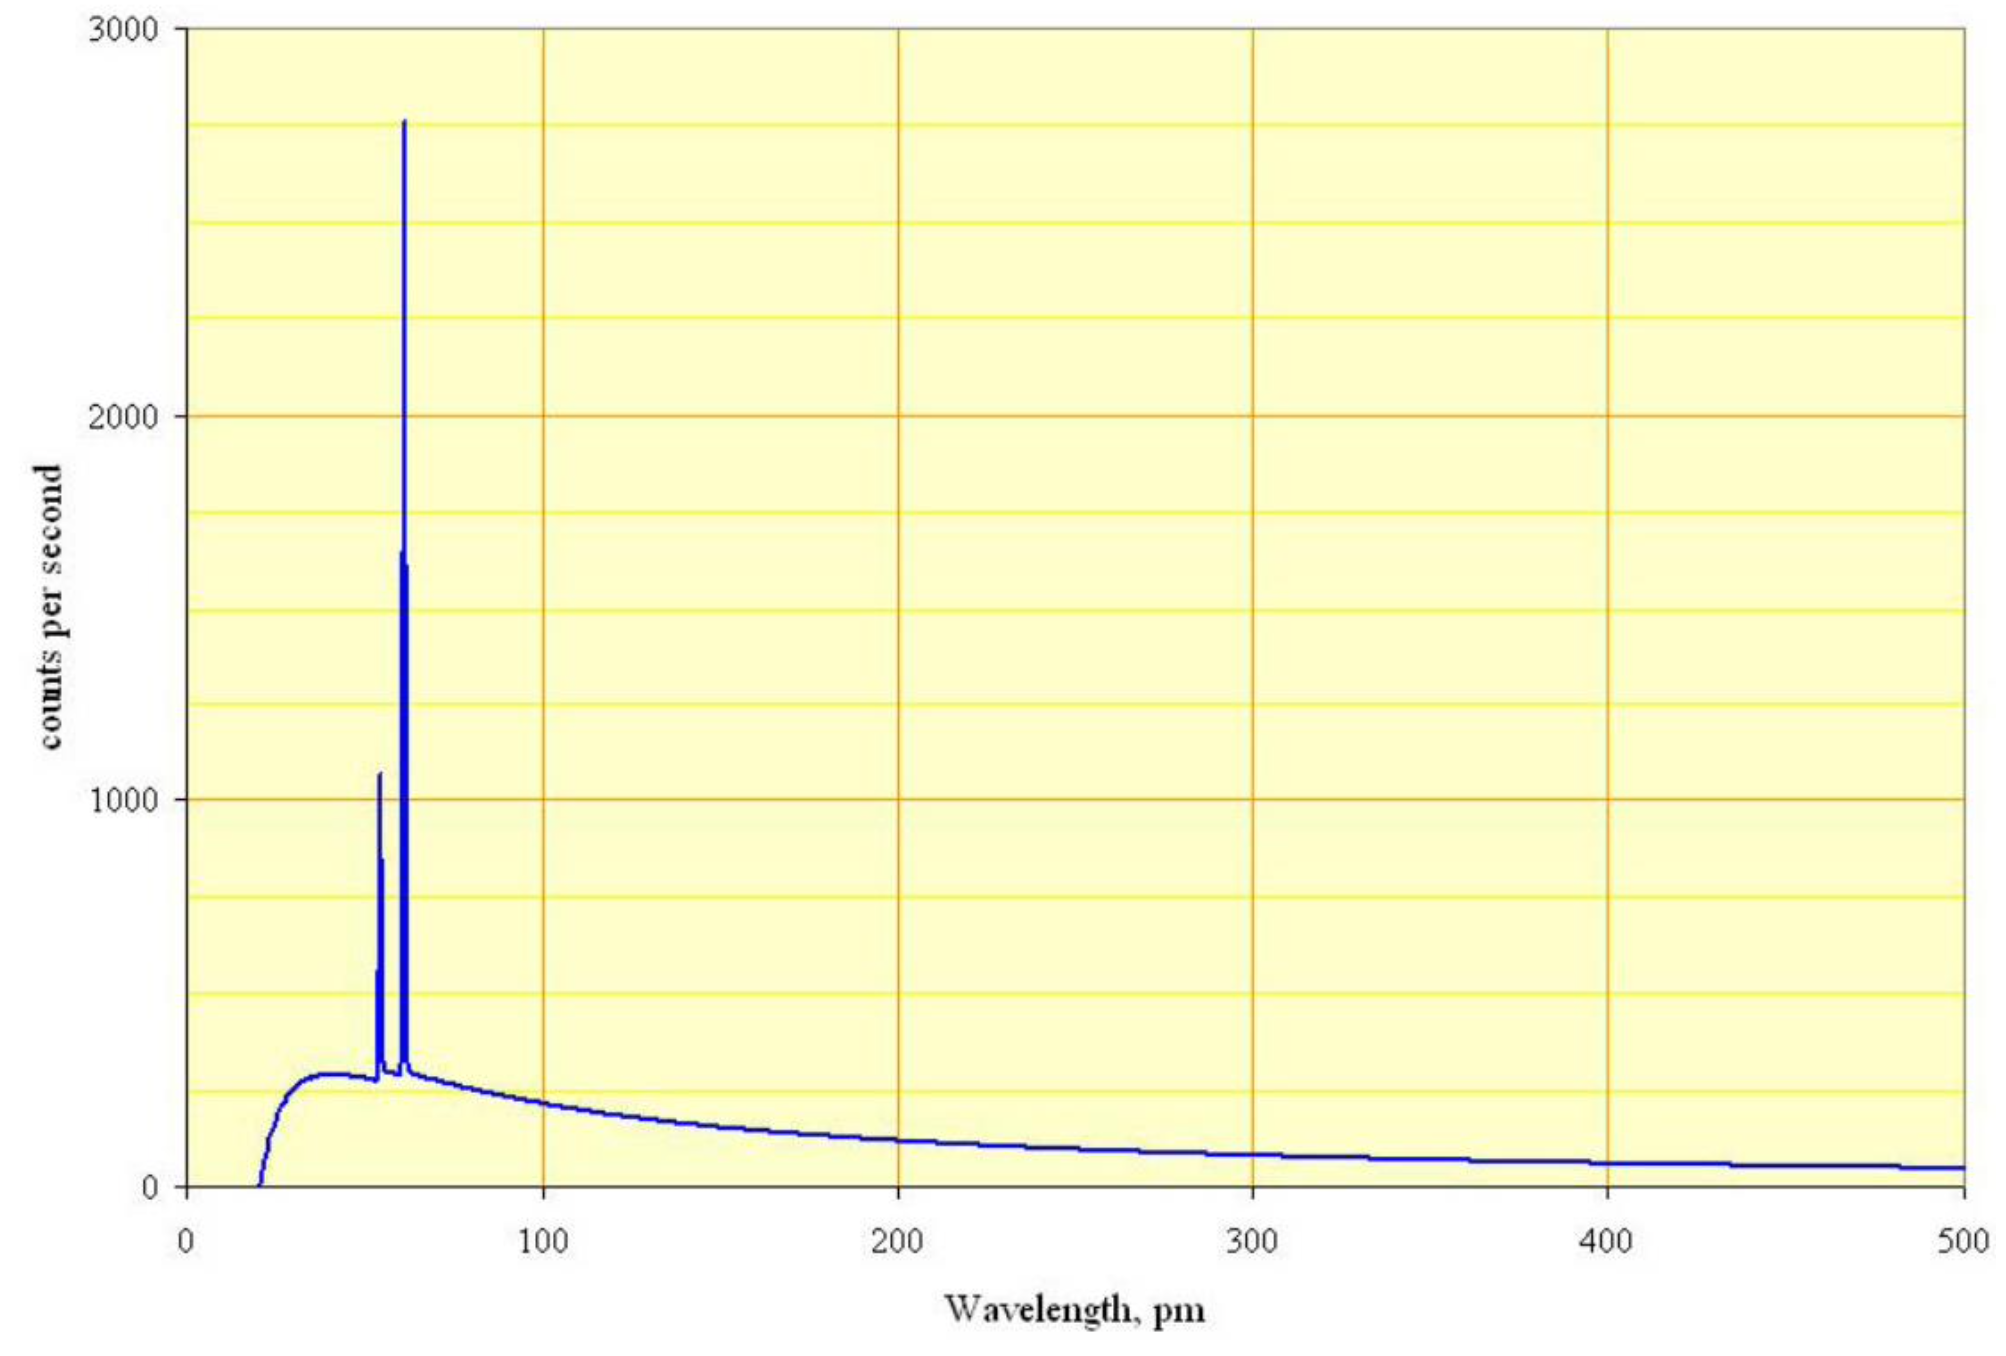
\includegraphics[width=0.5\linewidth]{xrayTubeSpectrum.png}
        \caption{The spectrum of X-rays generated in an X-ray tube.}
        \label{fig:xrayTubeSpectrum}
    \end{figure}
    \begin{itemize}
        \item The spectrum is a smooth, continuous curve with spikes.
        \item Implies two types of radiation: \textbf{Bremsstrahlung radiation} and \textbf{Characteristic radiation}.
        \item You want to get rid of the Bremsstrahlung radiation.
        \begin{itemize}
            \item The ultimate goal is to get your X-ray tube to emit only a single wavelength at high intensity, and the natural choice is the highest characteristic peak. Thus, everything else must go.
        \end{itemize}
    \end{itemize}
    \item \textbf{Bremsstrahlung radiation}: Electromagnetic radiation generated via deceleration of a charged particle when deflected by another charged particles (e.g., electrons by protons). \emph{Also known as} \textbf{braking radiation}, \textbf{continuous X-radiation}. \emph{Etymology} \textbf{bremsstrahlung} from German \emph{bremsen} "to brake" and \emph{strahlung} "radiation."
    \begin{figure}[h!]
        \centering
        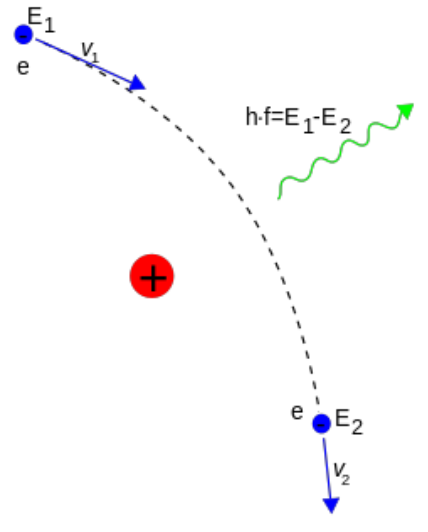
\includegraphics[width=0.16\linewidth]{generationBremsstrahlung.png}
        \caption{Generation mechanism for bremsstrahlung radiation.}
        \label{fig:generationBremsstrahlung}
    \end{figure}
    \begin{itemize}
        \item The charged particle loses kinetic energy via generation of photons (law of conservation of energy).
        \begin{itemize}
            \item How is this "inelastic scattering??" What does that even mean? Ask in OH.
        \end{itemize}
        \item If you work with high-Z (proton number) elements, these nuclei generate a rather strong electric fields.
        \item Strong electric fields scatter the electrons.
        \item The spectrum of these X-rays is continuous (hence the moniker "continuous X-rays").
        \item The frequency of bremsstrahlung radiation is limited by the energy of incident electrons.
        \item Peak intensity shifts toward higher frequencies when the energy of the decelerated particle (particle to be decelerated) increases.
        \item Peak intensity increases when the energy of the decelerated particle increases.
        \begin{itemize}
            \item Rationalizing these last two statements?? Ask in OH. Related to current and voltage below??
        \end{itemize}
    \end{itemize}
    \item X-ray notation for atomic energy levels.
    \begin{figure}[H]
        \centering
        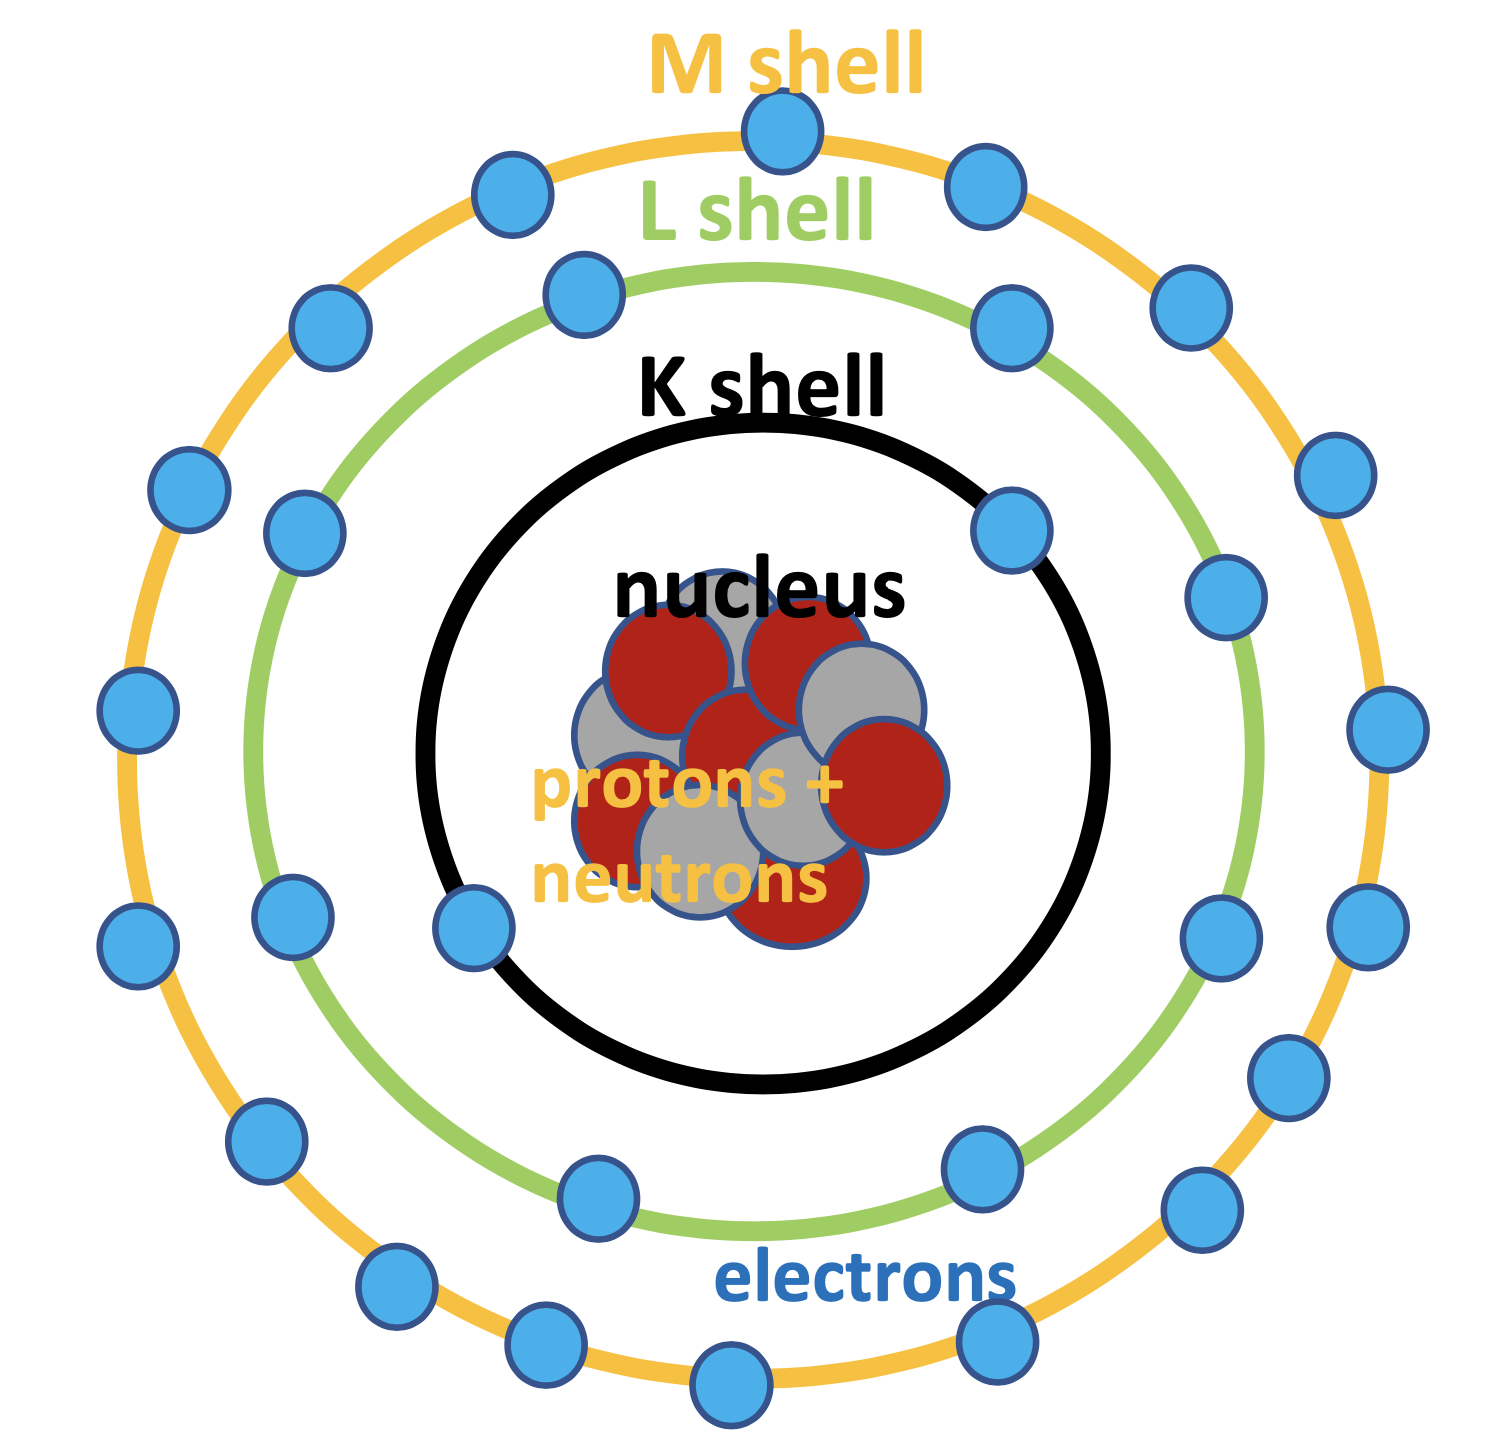
\includegraphics[width=0.3\linewidth]{bohrModel.png}
        \caption{Energy levels in the Bohr model.}
        \label{fig:bohrModel}
    \end{figure}
    \begin{itemize}
        \item The K, M, and L shells correspond to energy levels $n=1,2,3$, respectively.
        \item Somewhat antiquated notation from the early days of X-ray invention when the Bohr model was still popular.
    \end{itemize}
    \item Contribution of Bremsstrahlung.
    \begin{figure}[h!]
        \centering
        \begin{subfigure}[b]{0.49\linewidth}
            \centering
            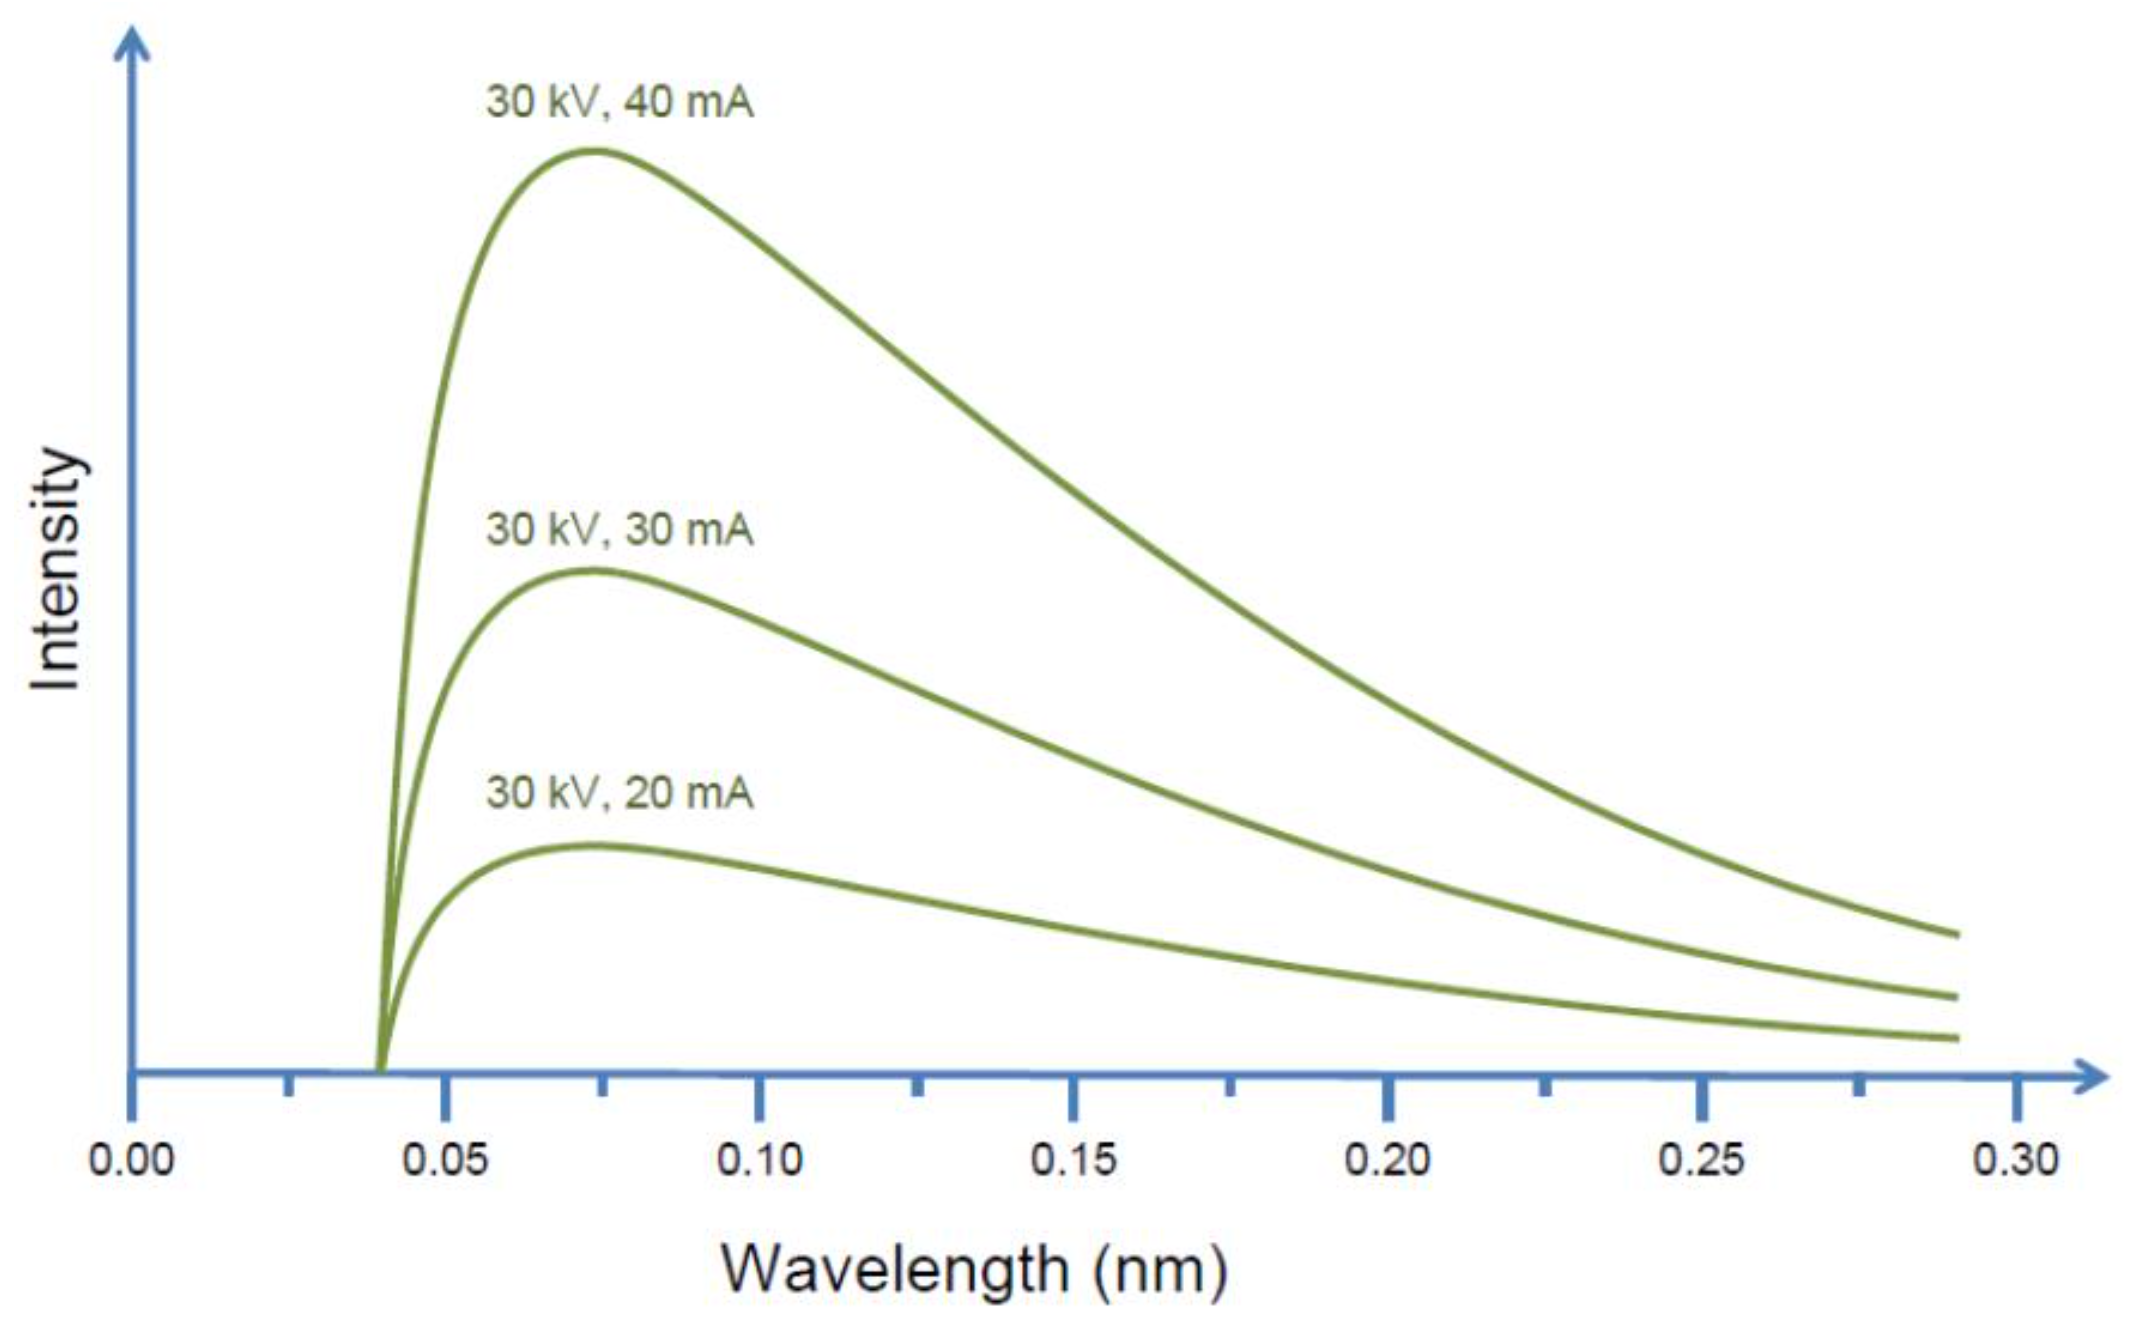
\includegraphics[width=0.8\linewidth]{xrayVoltageCurrenta.png}
            \caption{Varying current.}
            \label{fig:xrayVoltageCurrenta}
        \end{subfigure}
        \begin{subfigure}[b]{0.49\linewidth}
            \centering
            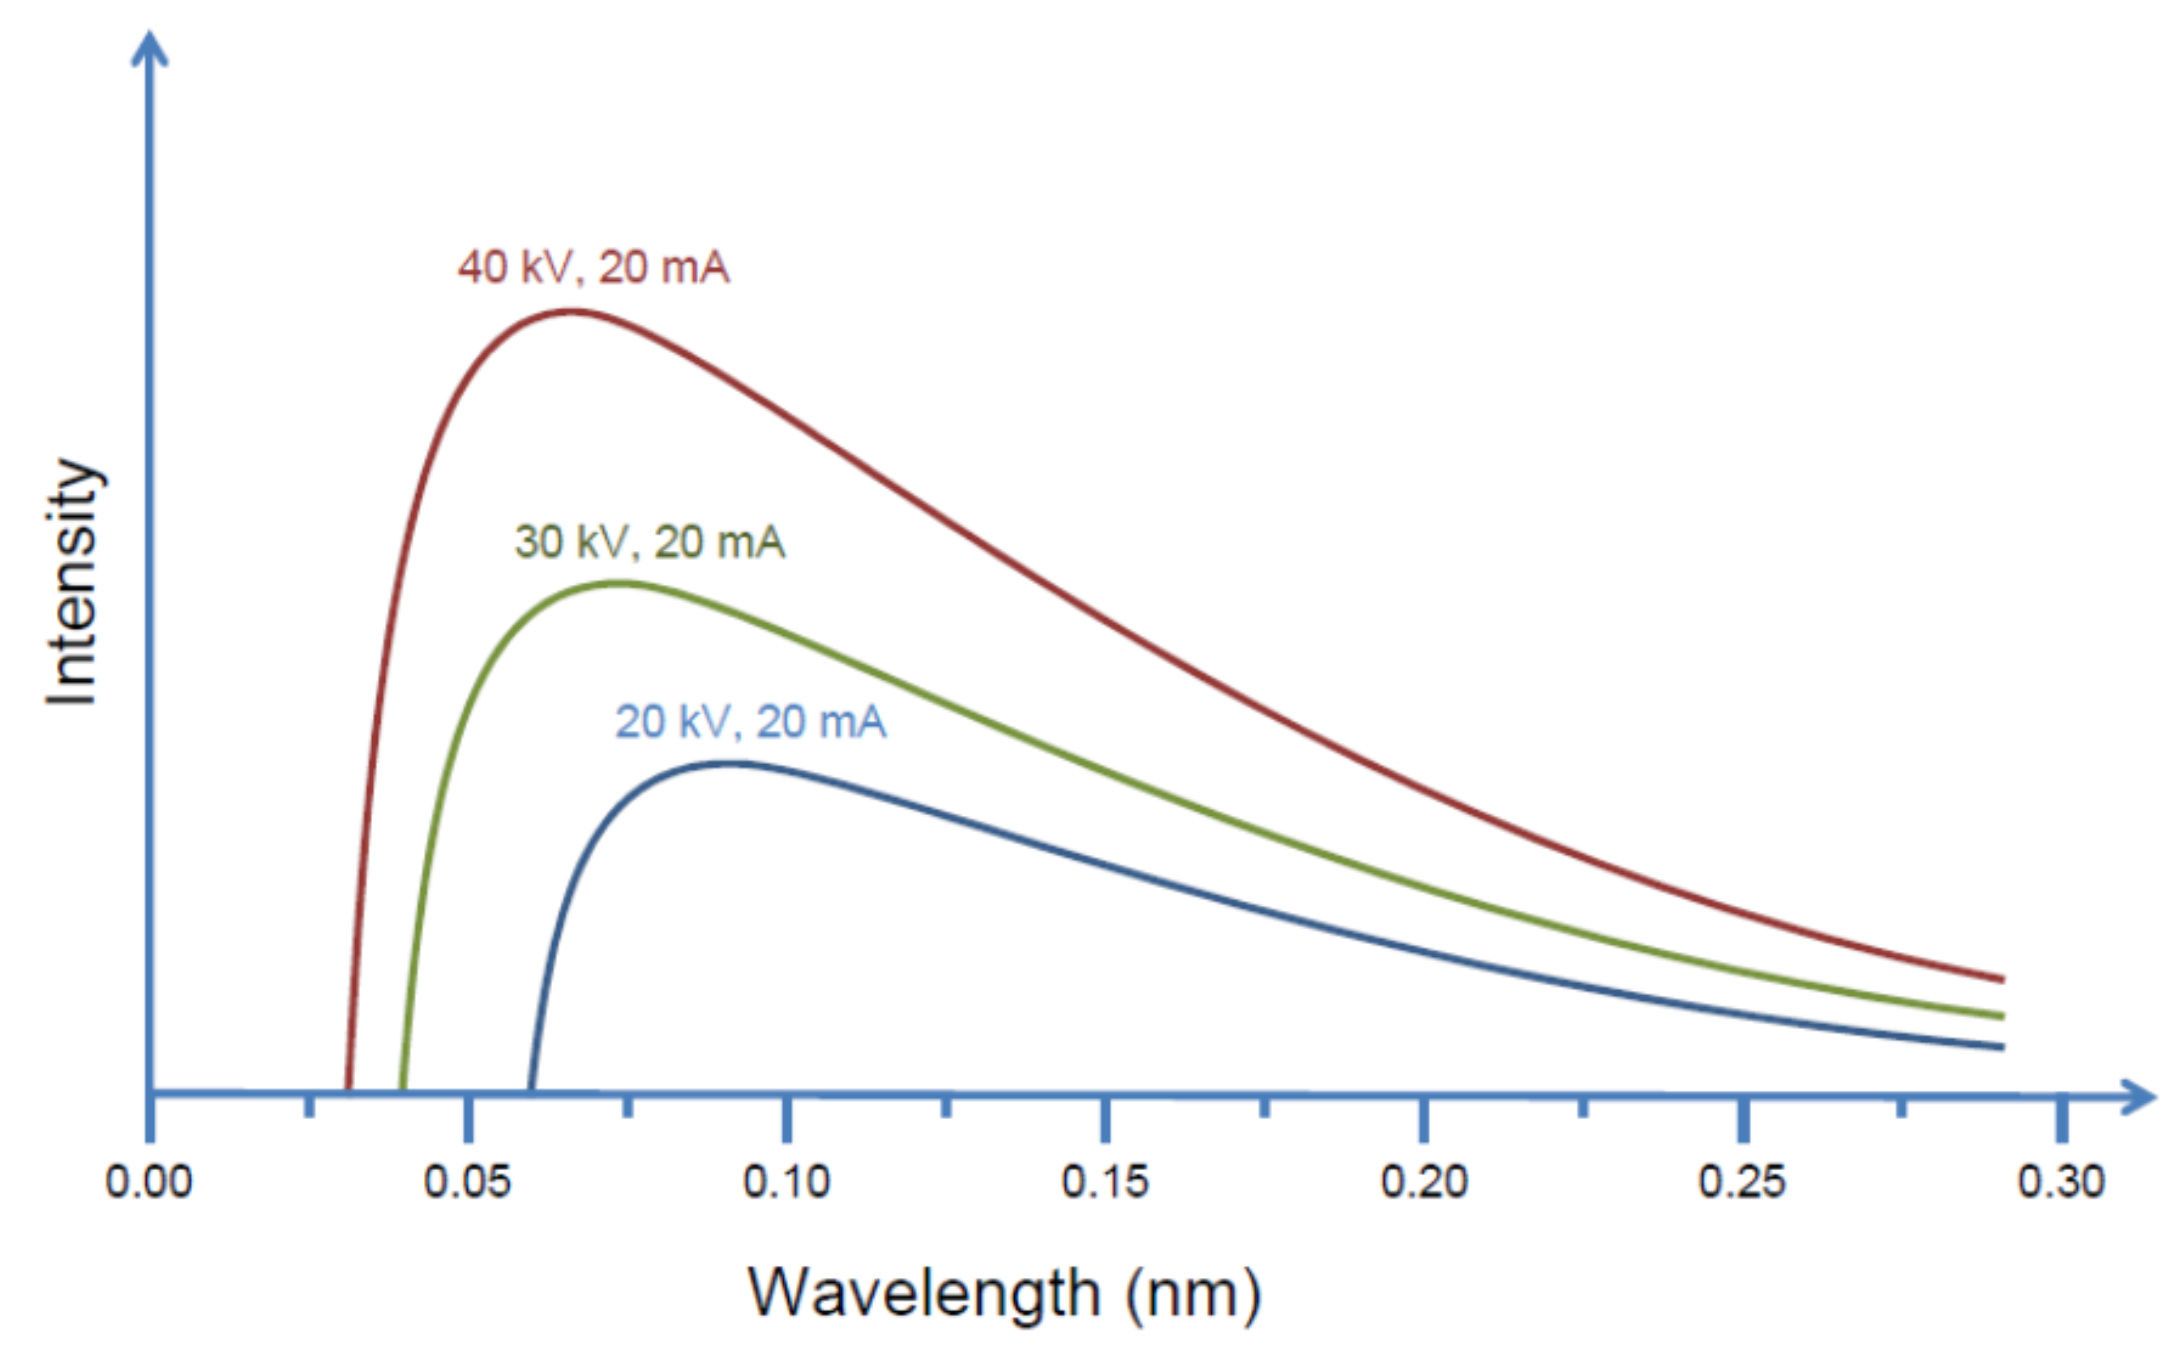
\includegraphics[width=0.8\linewidth]{xrayVoltageCurrentb.png}
            \caption{Varying voltage.}
            \label{fig:xrayVoltageCurrentb}
        \end{subfigure}
        \caption{X-ray intensity vs. wavelength at different voltages and currents.}
        \label{fig:xrayVoltageCurrent}
    \end{figure}
    \begin{itemize}
        \item The distribution of intensity (photon counts) against the wavelengths of the emitted radiation.
        \item Two settings you can change during the measurement: Current and voltage.
        \begin{itemize}
            \item When you increase the current, the intensity increases (more electrons means more counts per second).
            \item When you increase the voltage, the intensity increases and the peak shifts to higher frequencies (higher energy electrons means higher energy [resp. frequency] radiation).
        \end{itemize}
        \item See \textbf{Kramer's law} and its consequence the \textbf{Duane-Hunt law} for more on the functional form of these curves. Note that these curves are different from the Planck blackbody distribution law, even though they look somewhat similar.
    \end{itemize}
    \item \textbf{Kramer's law}: The law describing the spectral distribution of X-rays produced by electrons hitting a solid target. \emph{Given by}
    \begin{equation*}
        I(\lambda)\dd\lambda = K\left( \frac{\lambda}{\lambda_\text{min}}-1 \right)\cdot\frac{1}{\lambda^2}\dd\lambda
    \end{equation*}
    \begin{itemize}
        \item The proportionality constant $K$ is \textbf{contact}.
        \item $\lambda_\text{min}$ is the $x$-intercept in Figure \ref{fig:xrayVoltageCurrent}.
    \end{itemize}
    \item \textbf{Contact}: A quantity proportional to the atomic number of the target element. \emph{Denoted by} $\bm{K}$.
    \item \textbf{Duane-Hunt law}: The relationship between the voltage $V$ applied to an X-ray tube and the maximum fequency $f$ of the $x$-rays emitted from the target. \emph{Given by}
    \begin{equation*}
        f = \frac{Ve}{h}
    \end{equation*}
    \begin{itemize}
        \item Note: $e=\SI{1.602e-19}{\coulomb}$ is the electron charge and $h=\SI{6.626e-34}{\joule\second}$ is Planck's constant.
    \end{itemize}
    \item \textbf{Characteristic emission}: The emission of quantized photons with energy corresponding to the energy difference between higher and lower states in the target atoms.
    \item Mechanism of characteristic emission.
    \begin{figure}[h!]
        \centering
        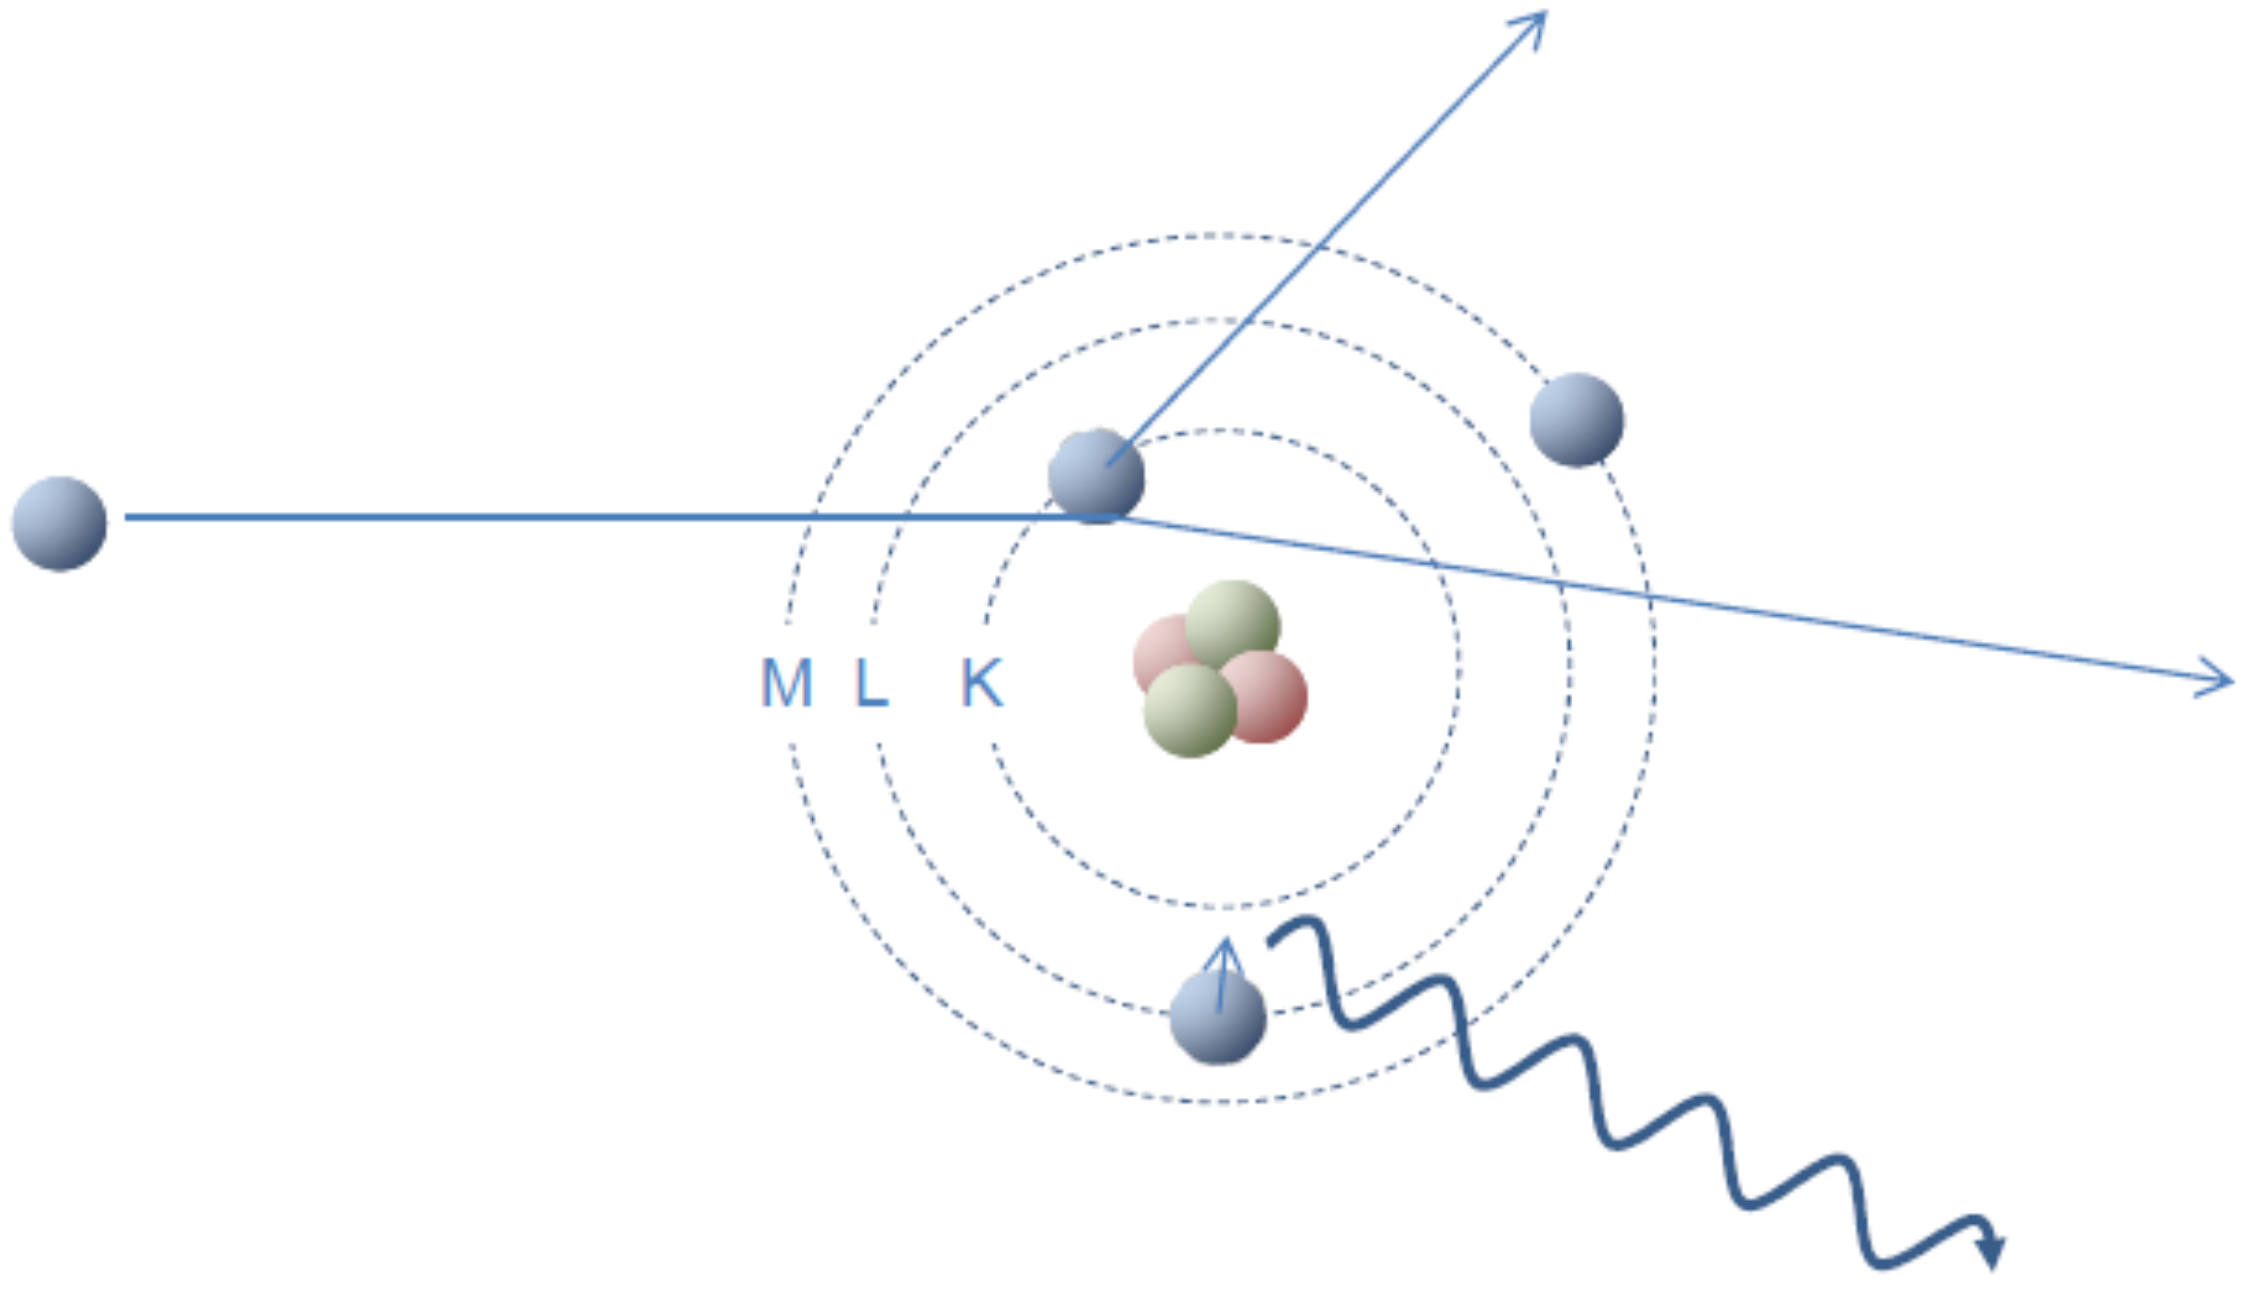
\includegraphics[width=0.5\linewidth]{generationCharacteristic.png}
        \caption{Generation mechanism for characteristic radiation.}
        \label{fig:generationCharacteristic}
    \end{figure}
    \begin{itemize}
        \item The target element is bombarded with high energy electrons.
        \item Incident electrons can knock orbital electrons out of the inner shell of the target atom.
        \item When this happens, the atom is left with a \textbf{core hole}.
        \item Outer shell electrons fill the vacancy, losing energy in the form of X-radiation to do so.
        \item Results in emissions characteristic of the target element (each element has unique energy levels).
        \item The maximum energy of the generated X-ray photon is limited by the energy of the incident electron, which is equal to the voltage on the tube times the electron charge.
    \end{itemize}
    \item \textbf{Core hole}: A vacant energy level in the core electron shell.
    \item We often use copper as the target element.
    \begin{figure}[H]
        \centering
        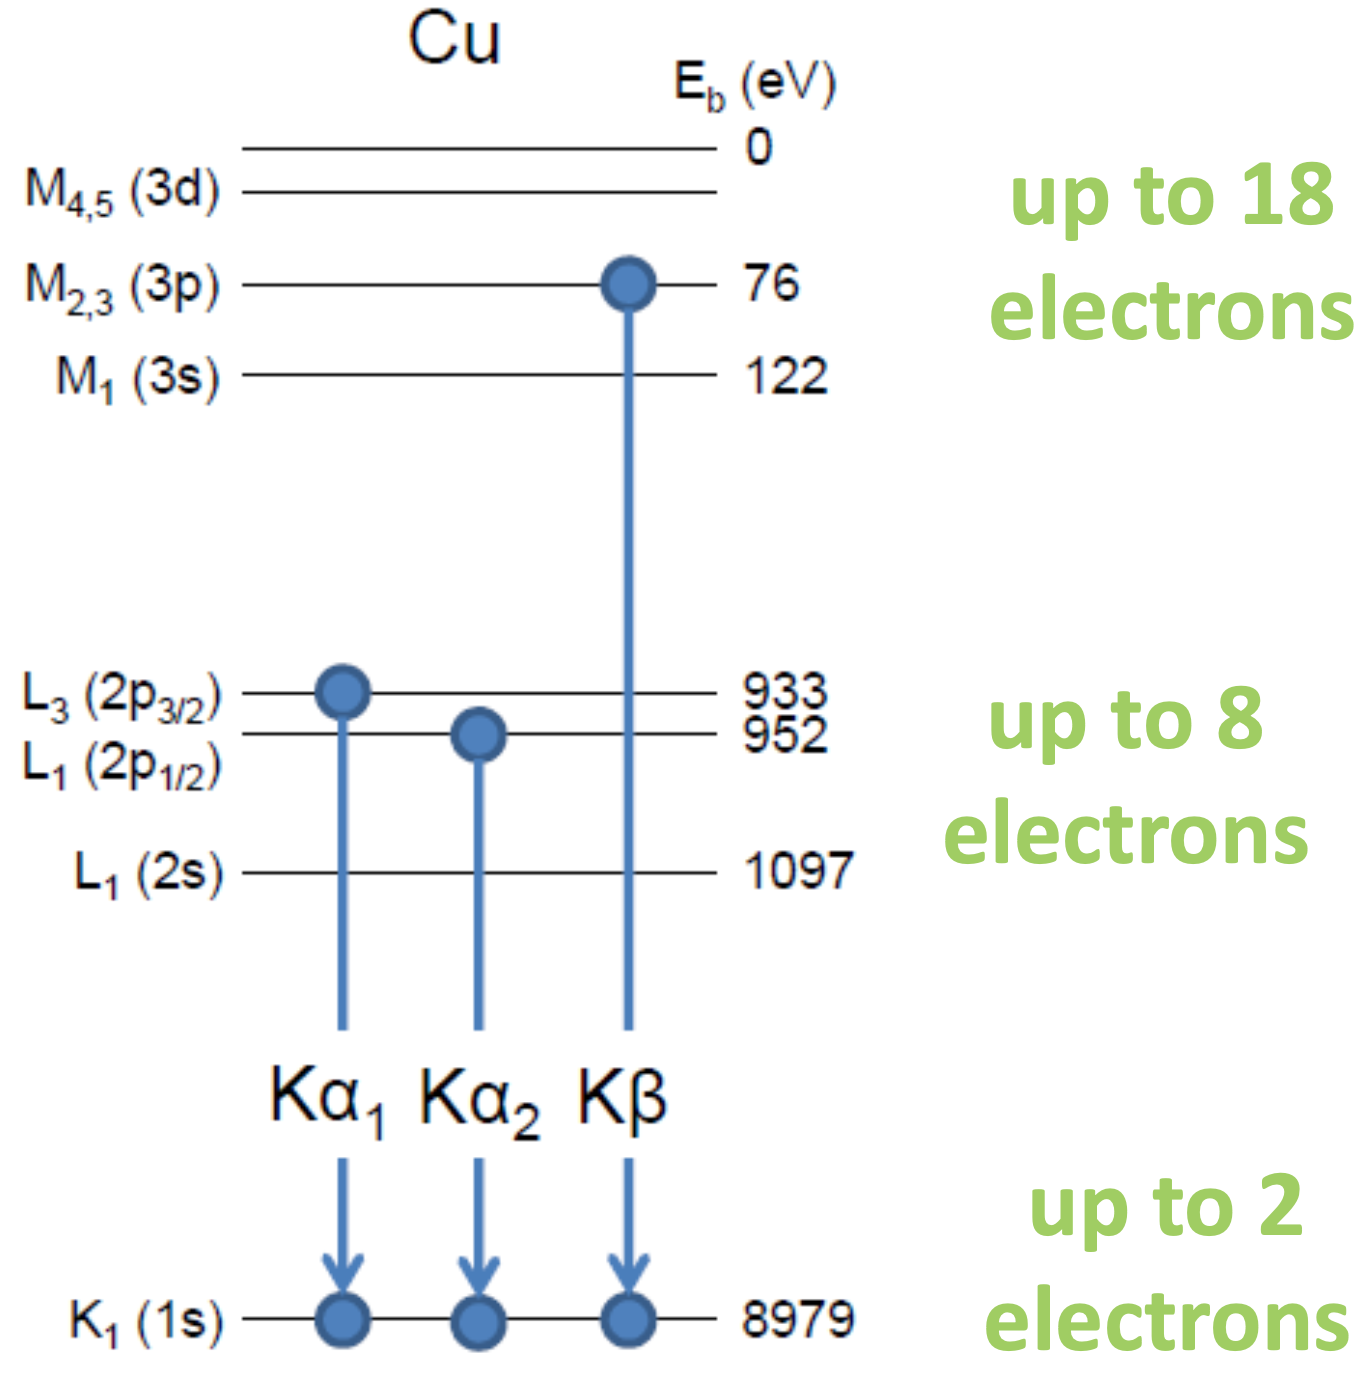
\includegraphics[width=0.3\linewidth]{copperCharacteristic.png}
        \caption{Copper spectral lines.}
        \label{fig:copperCharacteristic}
    \end{figure}
    \begin{itemize}
        \item The copper $K_\alpha$ line has greater intensity than the $K_\beta$ one and thus is more desirable in diffraction experiments.
        \item The same holds true in many elements, including the occasional alternative molybdenum.
    \end{itemize}
    \item Achieving monochromic emission.
    \begin{itemize}
        \item The X-rays are released from the anode with a range of energies.
        \begin{itemize}
            \item There are continuous X-rays produced by the X-ray tube, $K_\beta$ rays, and fluorescent X-rays from the sample.
        \end{itemize}
        \item Applications require monochormatic X-rays, so all of these (except the desired $K_\alpha$ ray) need to be filtered out.
        \item X-rays of undesirable energies can be filtered using \textbf{filters} and \textbf{monochromators}.
        \item You need filters to make the spectrum of X-rays really narrow??
    \end{itemize}
    \item X-ray filters.
    \begin{figure}[h!]
        \centering
        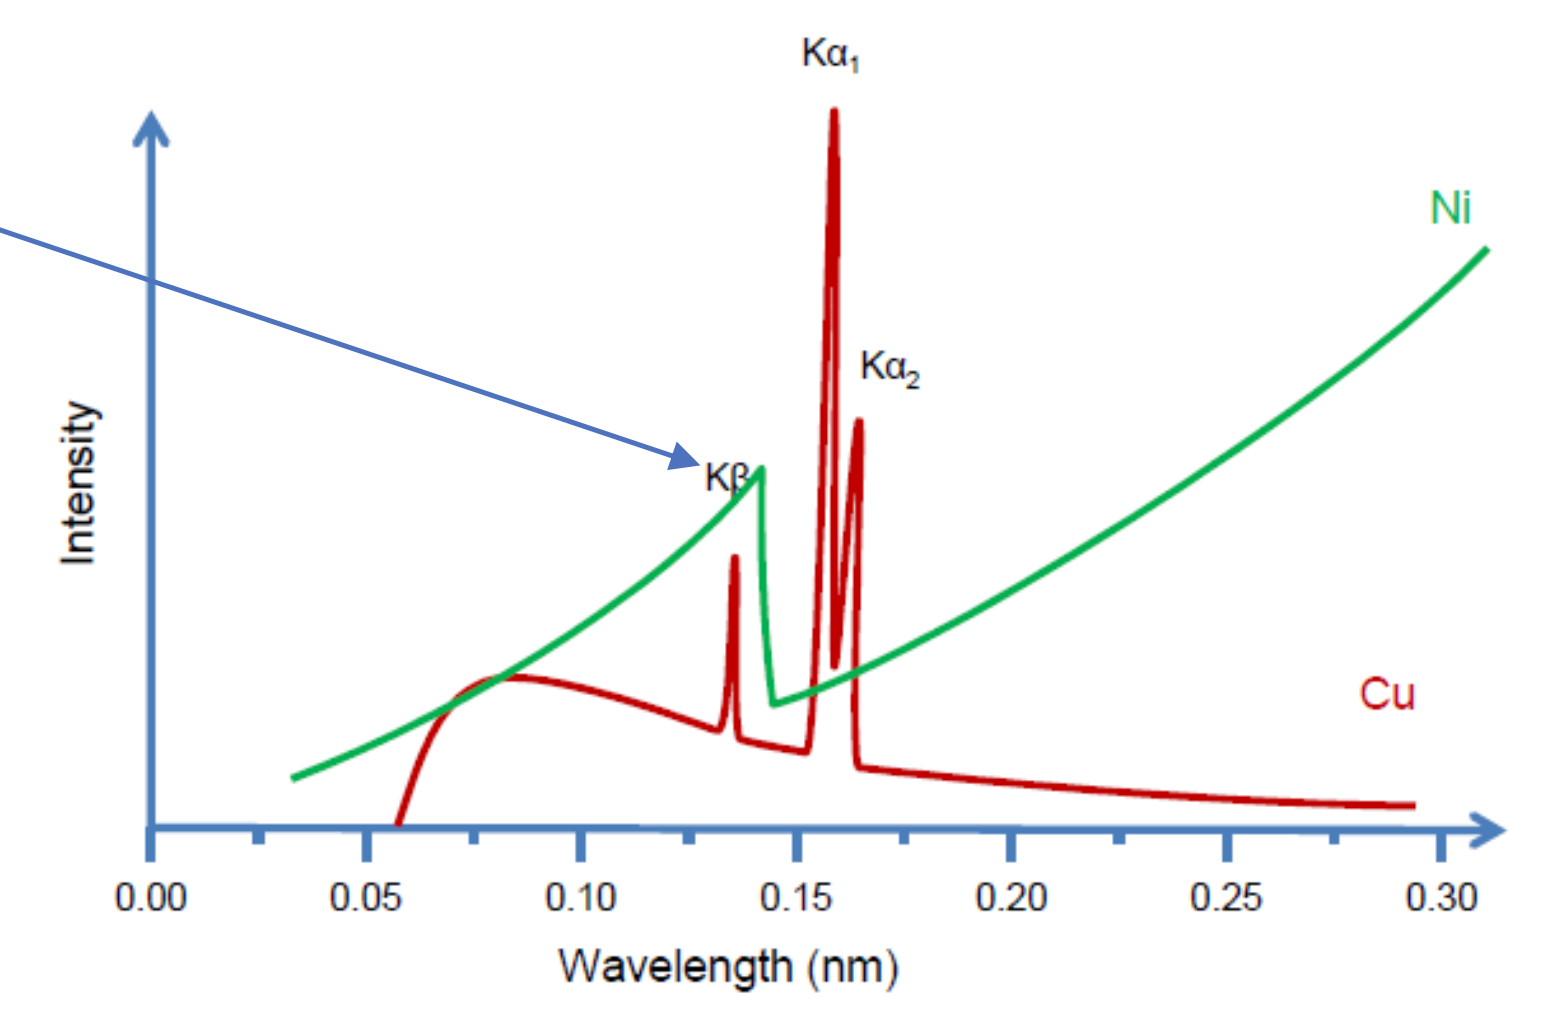
\includegraphics[width=0.5\linewidth]{NiFilter.png}
        \caption{Nickel filter for a copper anode.}
        \label{fig:NiFilter}
    \end{figure}
    \begin{itemize}
        \item The filter is usually nade of a metal that has one proton less than the anode material (e.g., \ce{Ni} filter for \ce{Cu} anode and \ce{Nb} filter for \ce{Mo} anode).
        \item Main purpose: To filter the $K_\beta$ line.
        \item The filtering of $K_\beta$ line depends on the thickness of the filter material.
        \item Example: The absorption edge of nickel metal is at \SI{1.488}{\angstrom}. This is between the $K_{\alpha_1}$ ($\lambda=\SI{1.542}{\angstrom}$) and $K_\beta$ ($\lambda=\SI{1.392}{\angstrom}$) X-ray spectral lines of copper. Hence, nickel foil of an appropriate thickness can be used to reduce the intensity of the \ce{Cu} $K_\beta$ line.
        \begin{itemize}
            \item In particular, nickel foil of thickness \SI{20}{\micro\meter} is typically used. It reduces the $K_\beta$ intensity by 99\% and the $K_\alpha$ intensity by only 58\%.
        \end{itemize}
    \end{itemize}
    \item X-ray targets.
    \begin{itemize}
        \item Most popular anode is \ce{Cu}, but can be \ce{Co} as well.
        \item \ce{Fe}, \ce{Cr}, and \ce{Mn} fluoresce under the incident Cu $K_\alpha$ beam, resulting in polychromatic radiation and alteration of the XRD results (strange shapes and elevated background).
        \begin{itemize}
            \item Implication: Be careful if you see something unusual in your spectra. We may not have won a Nobel prize for something novel; it could just be \ce{Fe}, \ce{Cr}, or \ce{Mn} contamination of the sample.
        \end{itemize}
        \item In this case, seek out an instrument that doesn't use \ce{Cu} or \ce{Co} as the target element.
        \begin{itemize}
            \item Or is it that we want to switch from \ce{Cu} to \ce{Co} in this case??
        \end{itemize}
    \end{itemize}
    \item Monochromators.
    \begin{itemize}
        \item Main purpose: To remove all X-rays but the $K_\alpha$ ones.
        \item The monochromator is a crystal.
        \item The monochromator works by reflecting wavelengths that obey Bragg's Law (see next lecture and \textcite{bib:CHEM26300Notes}) for the particular $d$ spacings of the monochromator.
        \item Desired characteristics.
        \begin{itemize}
            \item The crystals should have suitable interplanar distances $d$ so that the desired wavelength $\lambda$ can be obtained.
            \item The crystals must be mechanically strong and stable in the beam. This is why graphite and silicon are so popular.
            \item Low absorbance of X-rays (we are interested in reflection).
            \item Easy to grow single crystals at a reasonable cost.
        \end{itemize}
        \item Examples: pyrolytic graphite crystals, \ce{Si}, \ce{Ge}, \ce{LiF}, and \ce{LiCl}.
        \begin{itemize}
            \item PG crystals and Si are particularly popular choices.
            \item Graphite is a broad band monochromator: The variance around the allowed $\lambda$ is relatively large due to its \textbf{mosaicity}.
            \item In contrast, silicon is a narrow band monochromator.
        \end{itemize}
        \item With copper, the Bragg equation gives a very small difference in Bragg angle between $K_{\alpha_1}$ and $K_{\alpha_2}$. Thus, we need a narrow band monochromator such as \ce{Si}.
    \end{itemize}
    \item \textbf{Mosaicity}: The spread of crystal plane orientations.
    \begin{itemize}
        \item Essentially, less perfect crystals have planes that aren't perfectly aligned, creating spread.
    \end{itemize}
    \item Effect of monochromators.
    \begin{figure}[h!]
        \centering
        \begin{subfigure}[b]{0.49\linewidth}
            \centering
            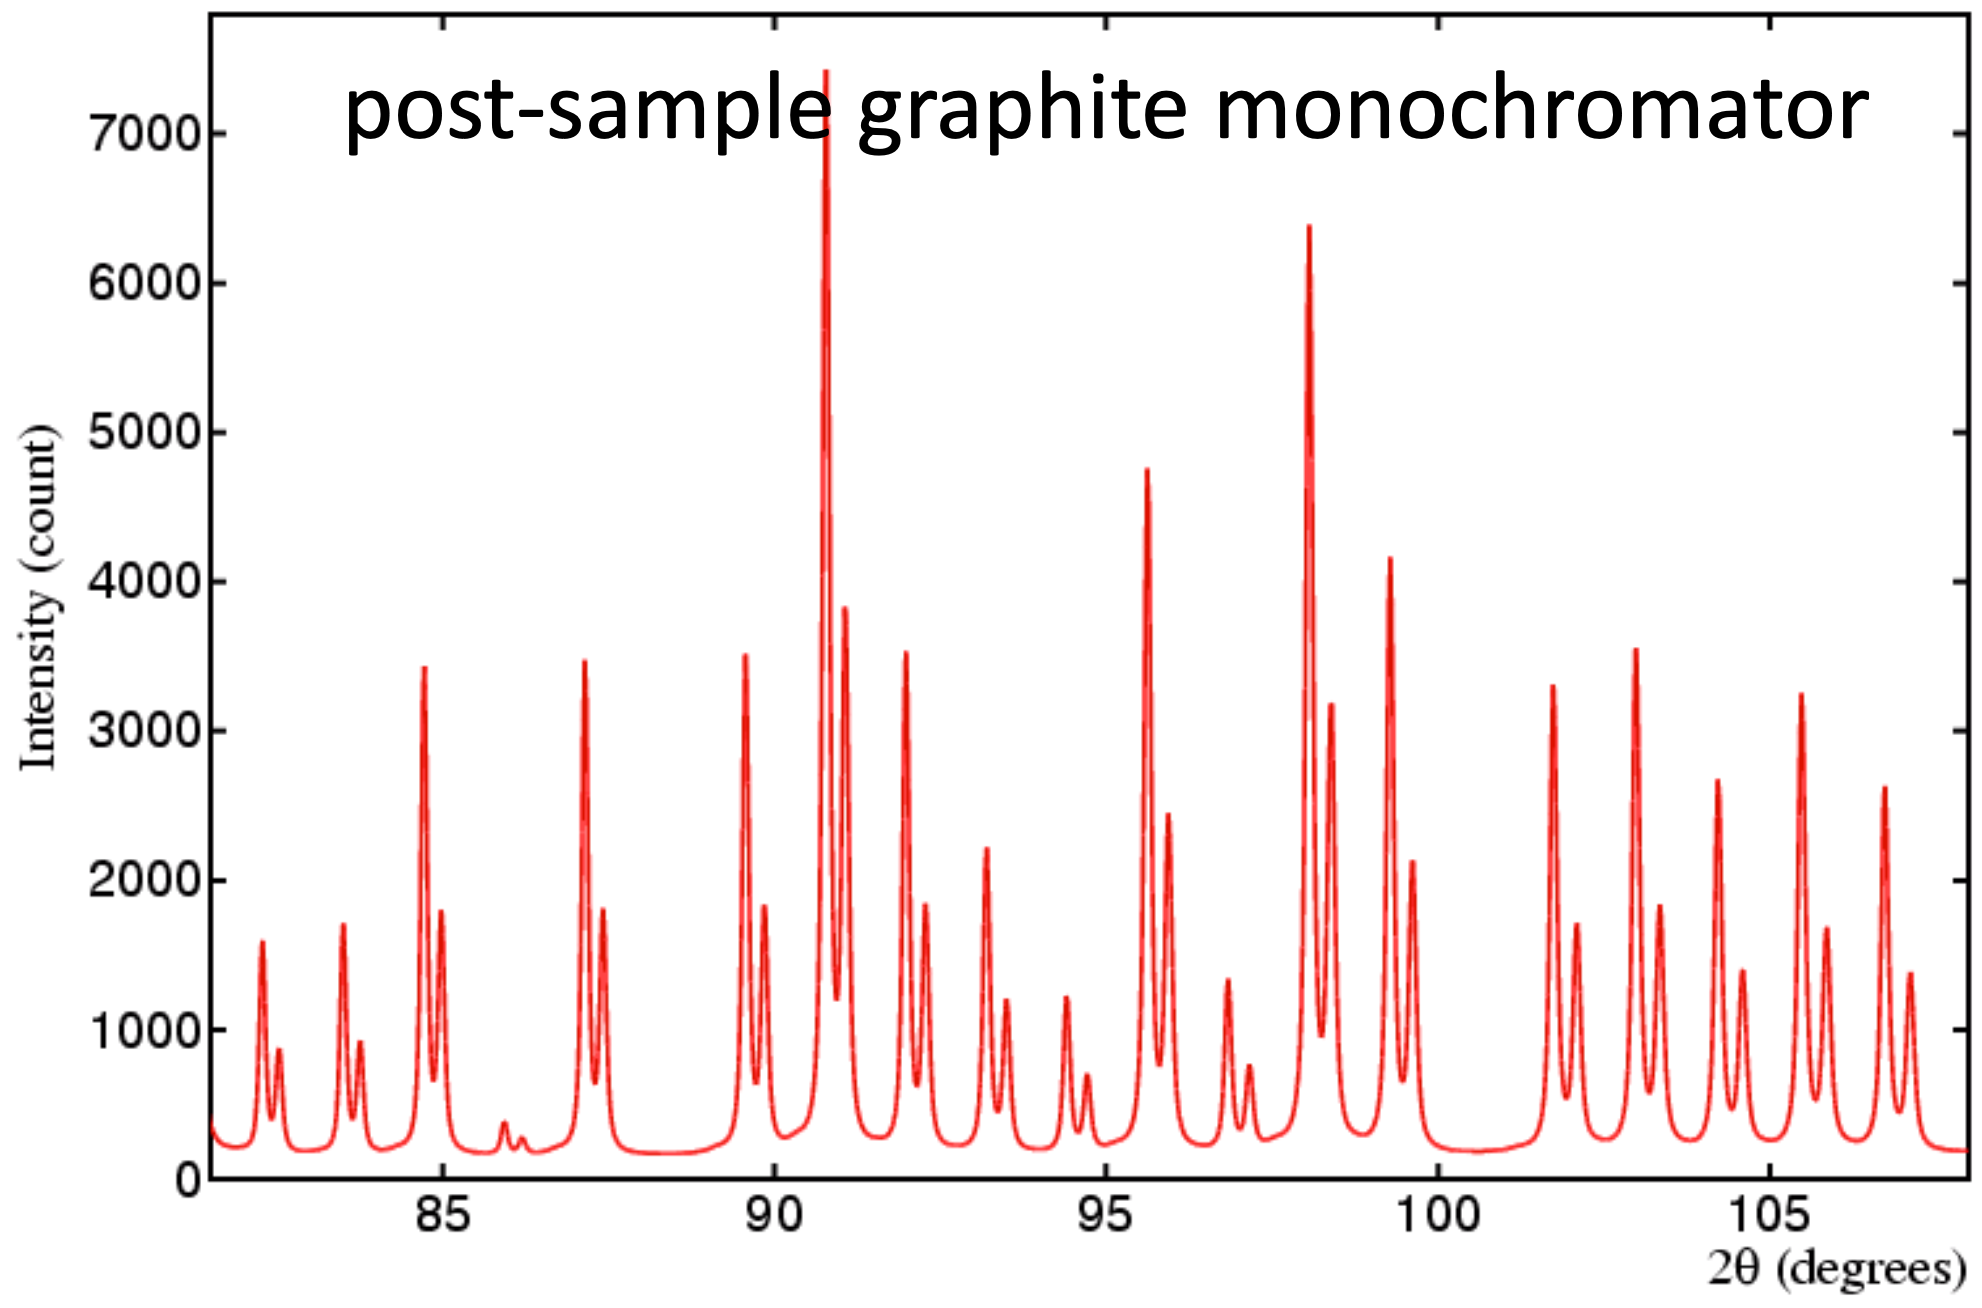
\includegraphics[width=0.8\linewidth]{monochromatorBeforeAftera.png}
            \caption{Broad band after.}
            \label{fig:monochromatorBeforeAftera}
        \end{subfigure}
        \begin{subfigure}[b]{0.49\linewidth}
            \centering
            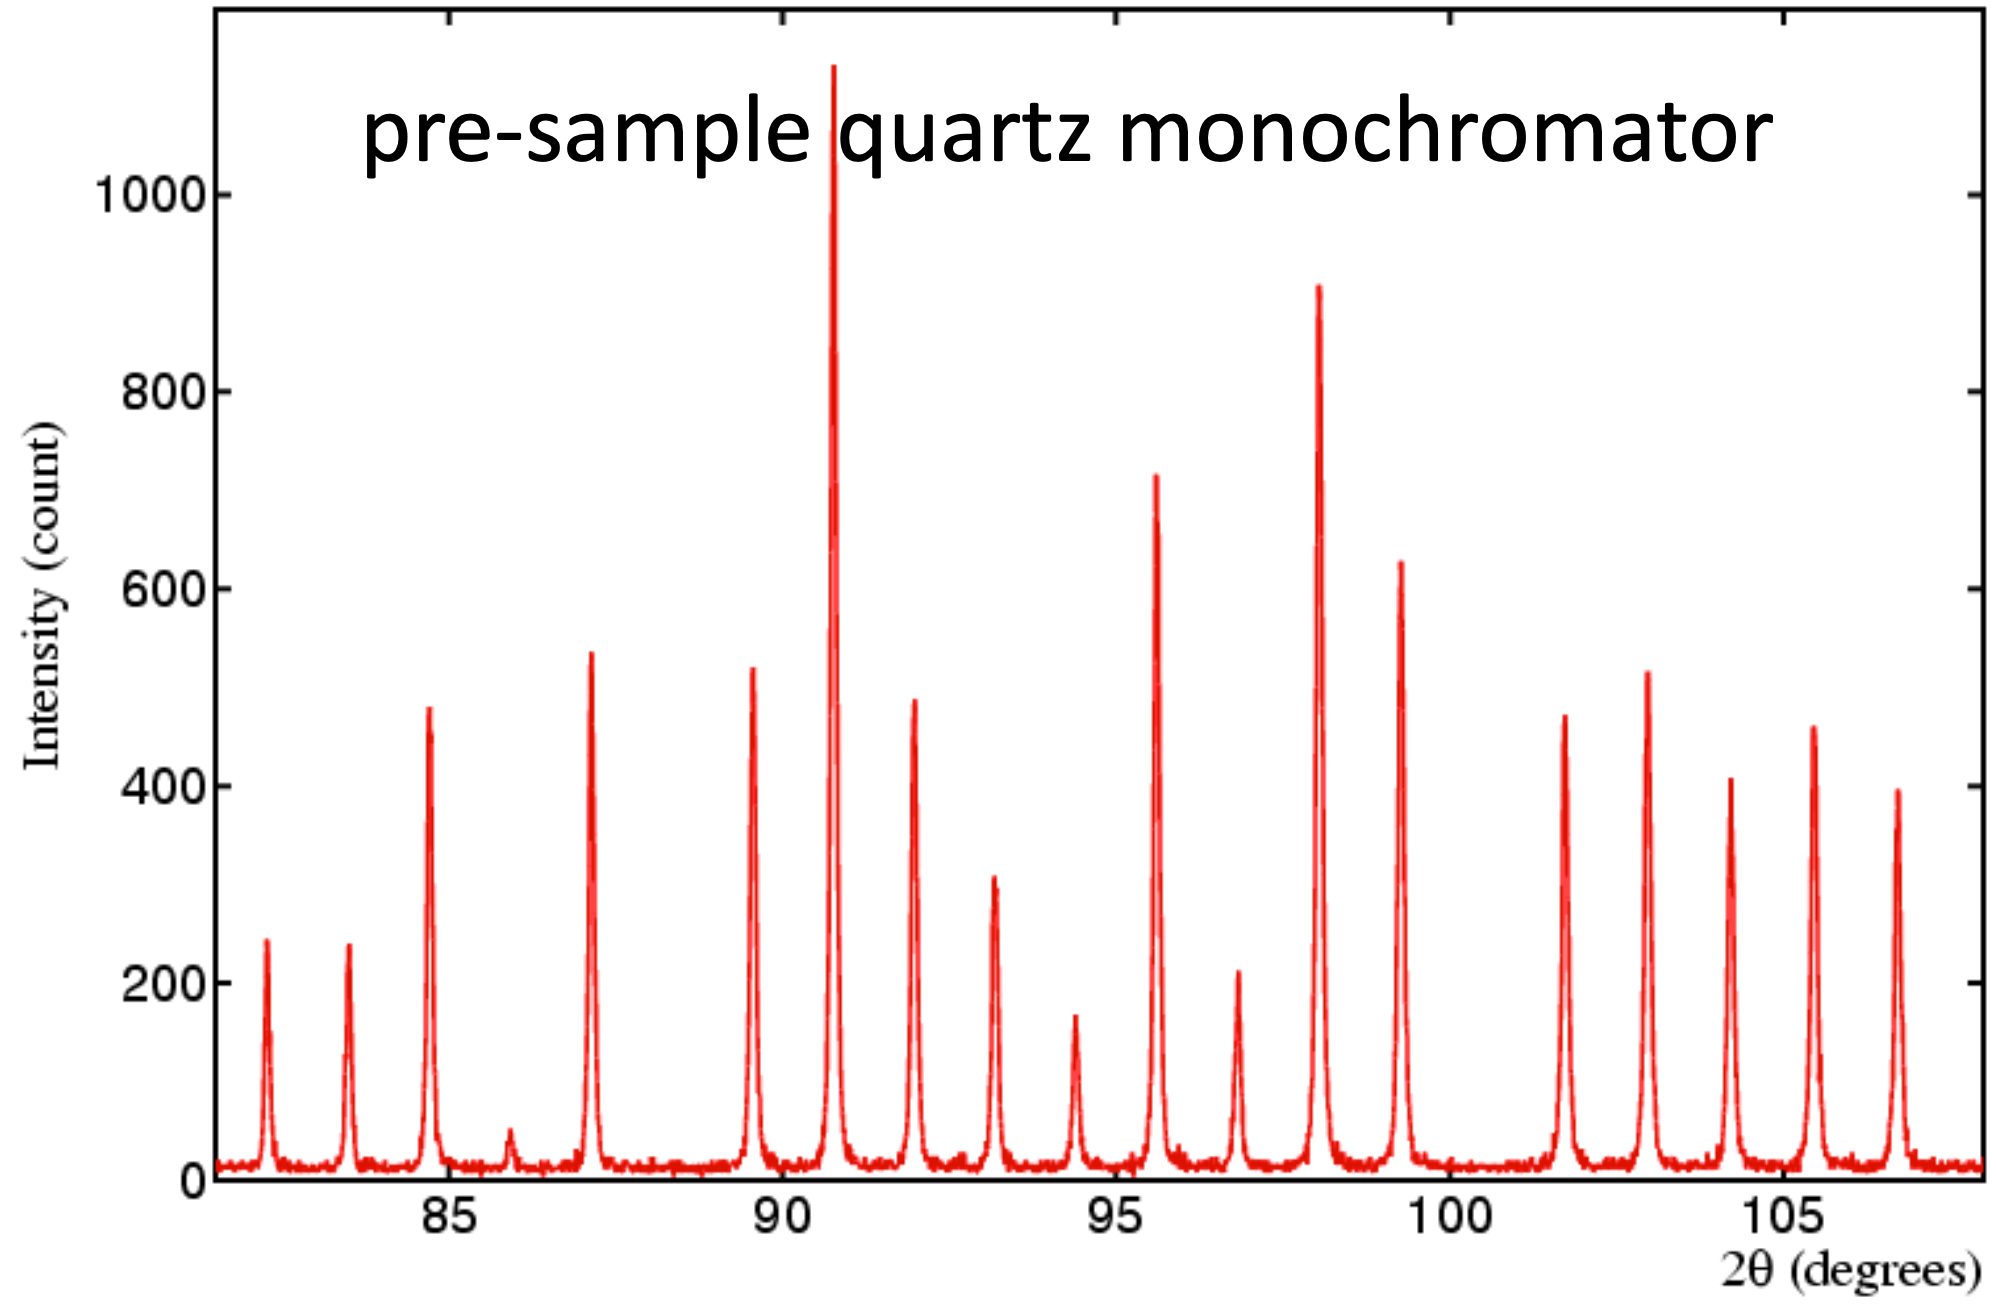
\includegraphics[width=0.8\linewidth]{monochromatorBeforeAfterb.png}
            \caption{Narrow band before.}
            \label{fig:monochromatorBeforeAfterb}
        \end{subfigure}
        \caption{Effect of monochromator type and placement.}
        \label{fig:monochromatorBeforeAfter}
    \end{figure}
    \begin{itemize}
        \item Monochromators can be placed before or after the sample.
        \item Most instruments have both.
        \item The spectrum in Figure \ref{fig:monochromatorBeforeAftera} was collected using a broad band monochromator after the sample.
        \begin{itemize}
            \item Splitting of the diffraction peaks is due to the presence of both $K_{\alpha_1}$ and $K_{\alpha_2}$ radiation.
        \end{itemize}
        \item The spectrum in Figure \ref{fig:monochromatorBeforeAfterb} was collected using a narrow band monochromator before the sample.
        \begin{itemize}
            \item Benefit: The peaks due to $K_{\alpha_2}$ radiation are removed.
            \item Drawback: Diffraction intensity is decreased.
        \end{itemize}
    \end{itemize}
    \item Working principle of the monochromator.
    \begin{itemize}
        \item Monochromators work based on Bragg's law ($\lambda=2d\sin\theta$) for the particular $d$ spacings of the monochromator.
        \item Let's investigate how a silicon monochromator can select for the $K_{\alpha_1}$ line of copper.
        \begin{itemize}
            \item Silicon has a cubic crystalline lattice with side length \SI{0.543}{\nano\meter}.
            \item Thus, the spacing of the 111 planes is
            \begin{equation*}
                d_{111} = \sqrt{\frac{0.543^2}{1^2+1^2+1^2}} = \SI{0.3135}{\nano\meter}
            \end{equation*}
            \item Using this value and the known wavelengths of the copper $K_{\alpha_1}$ and $K_{\alpha_2}$ lines (i.e., $\lambda=\SI{154.051}{\pico\meter},\SI{154.433}{\pico\meter}$, respectively), we can use Bragg's law to calculate the angle $2\theta$ at which we should orient the silicon 111 planes relative to the incident X-rays in order to select for one line or the other. In particular, if we want to select for the copper $K_{\alpha_1}$ line, we should use the angle of incidence
            \begin{equation*}
                2\theta = 2\sin^{-1}\left( \frac{\lambda}{2d} \right)
                = 2\sin^{-1}\left( \frac{\SI{154.051}{\pico\meter}}{2\cdot\SI{313.5}{\pico\meter}} \right)
                \approx \ang{28.442}
            \end{equation*}
            \item Owing to its high crystalline purity (low mosaicity), silicon at this angle can select for the desired wavelength.
        \end{itemize}
        \item Graphite monochromators will pass both $K_\alpha$ wavelengths, but not $K_\beta$ for which the Bragg angle is considerably different.
        \item Silicon has a peak position at 28.46. This number is right between the copper peaks; thus, it can separate the $K_{\alpha_1}$ and $K_{\alpha_2}$ wavelenghts from a laboratory X-ray source??
        \item Is this all correct??
    \end{itemize}
    \item Filters vs. monochromators.
    \begin{figure}[h!]
        \centering
        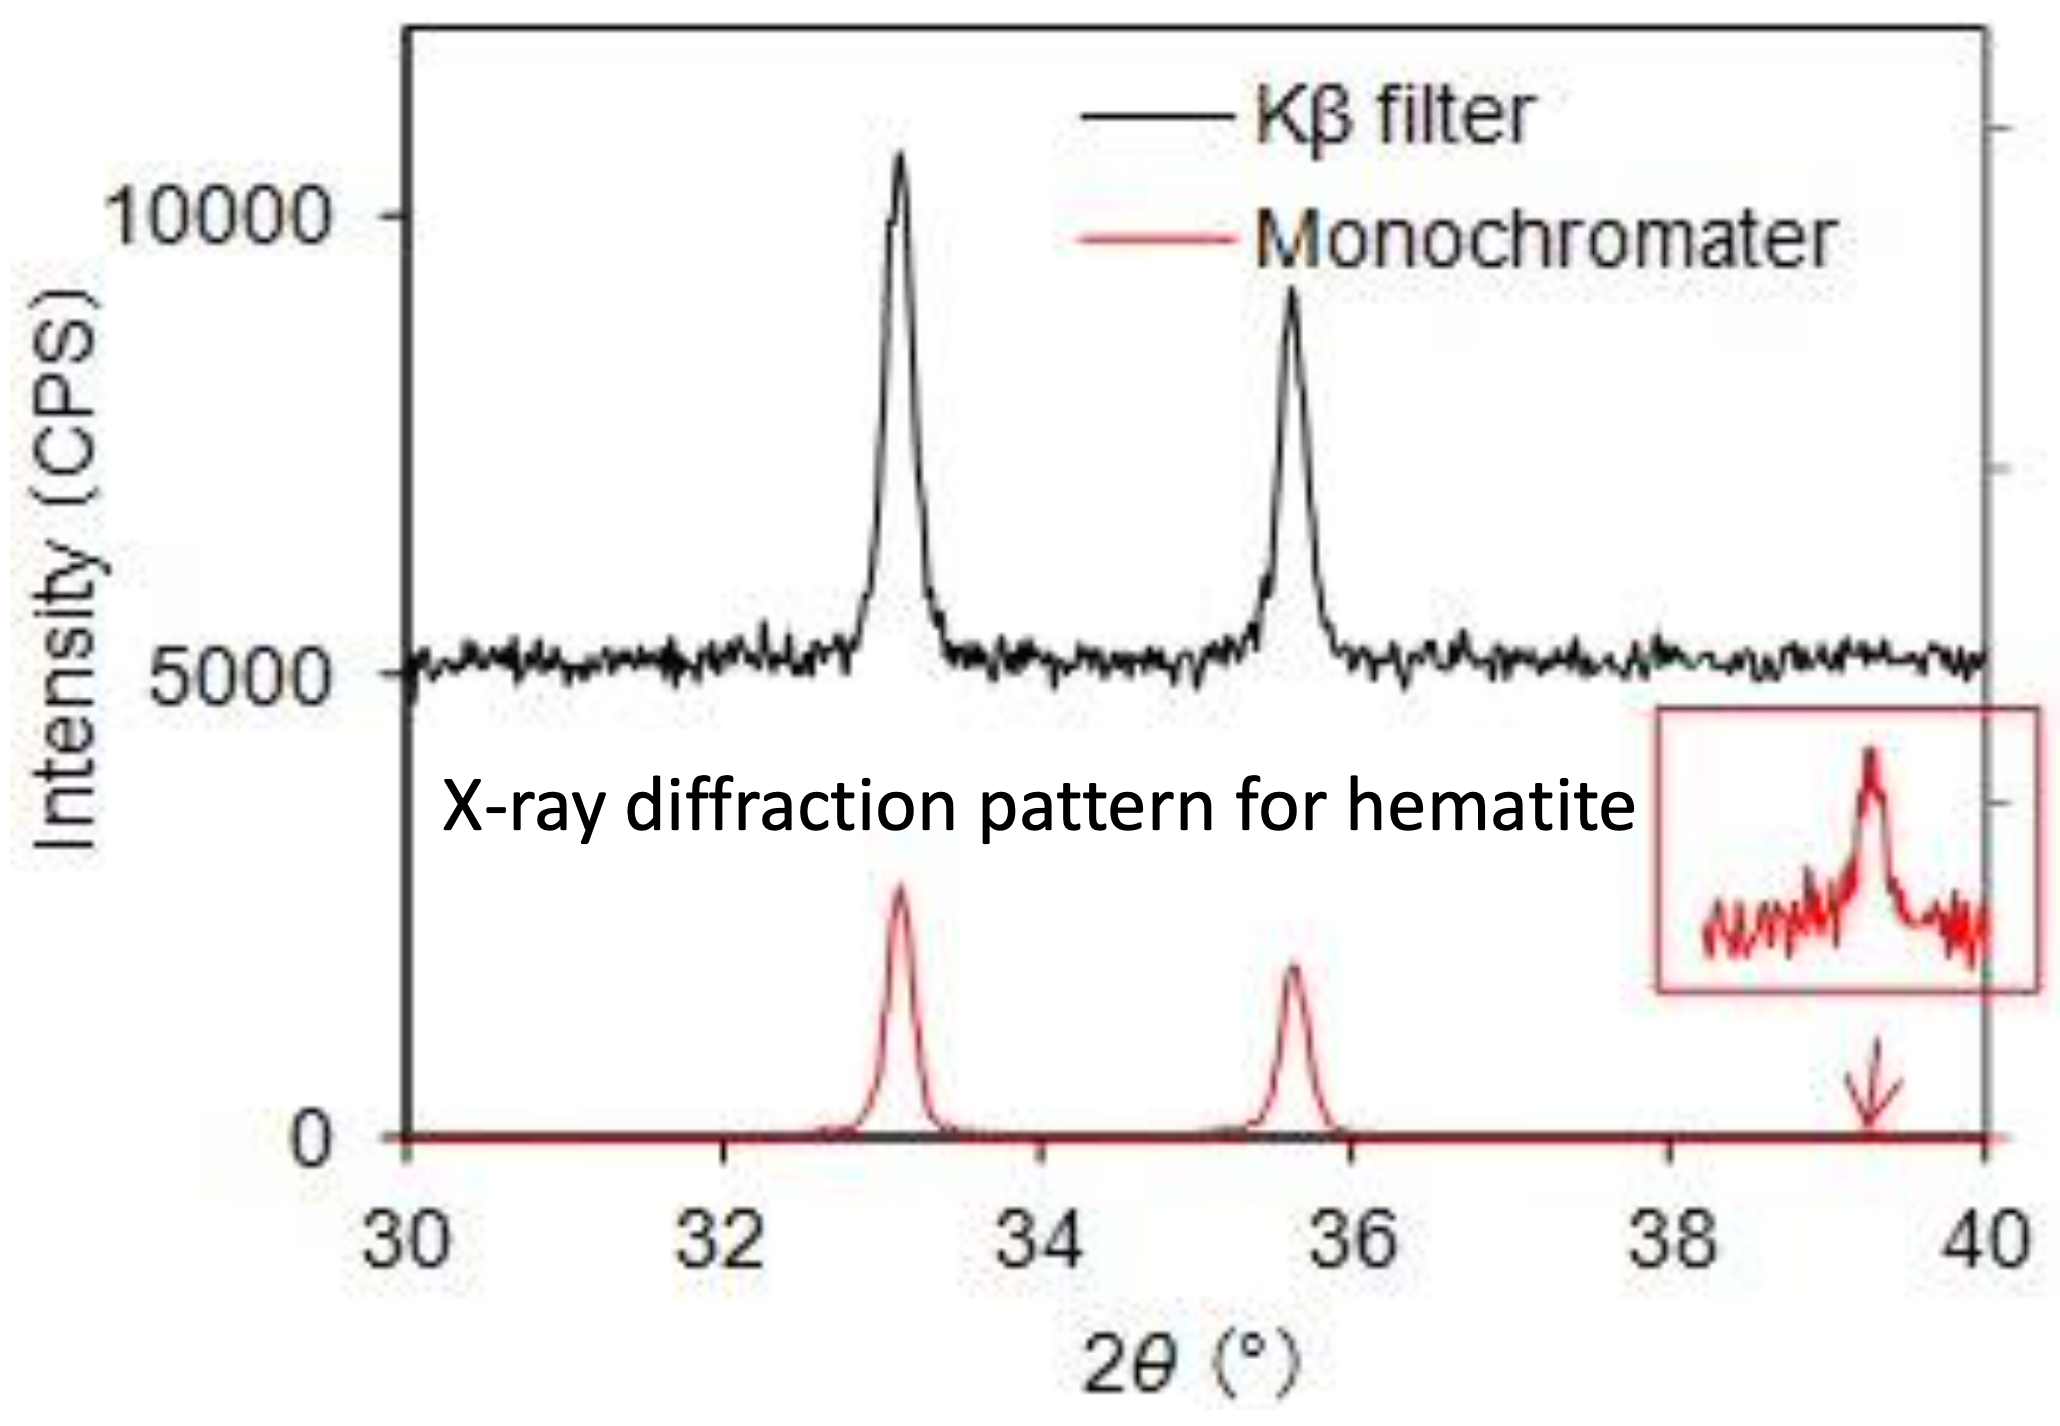
\includegraphics[width=0.45\linewidth]{filterVsMonochromator.png}
        \caption{Filters vs. monochromators.}
        \label{fig:filterVsMonochromator}
    \end{figure}
    \begin{itemize}
        \item Metal filter vs. a crystal monochromator.
        \item By using a monochromator, it is possible to obtain X-ray diffraction patterns with high signal-to-background ratios since the monochromator can remove interfering components such as continuous X-rays produced by the X-ray tube, $K_\beta$ rays, and fluorescent X-rays from the sample.
        \item Notice the extra noise in the spectrum taken with a $K_\beta$ filter in Figure \ref{fig:filterVsMonochromator}.
        \item One nice thing about using a filter, though, is that you preserve more intensity (monochromators rely on relatively low-probability reflection events as opposed to high probability transmission events).
    \end{itemize}
    \item Beam divergence.
    \begin{figure}[H]
        \centering
        \begin{subfigure}[b]{0.3\linewidth}
            \centering
            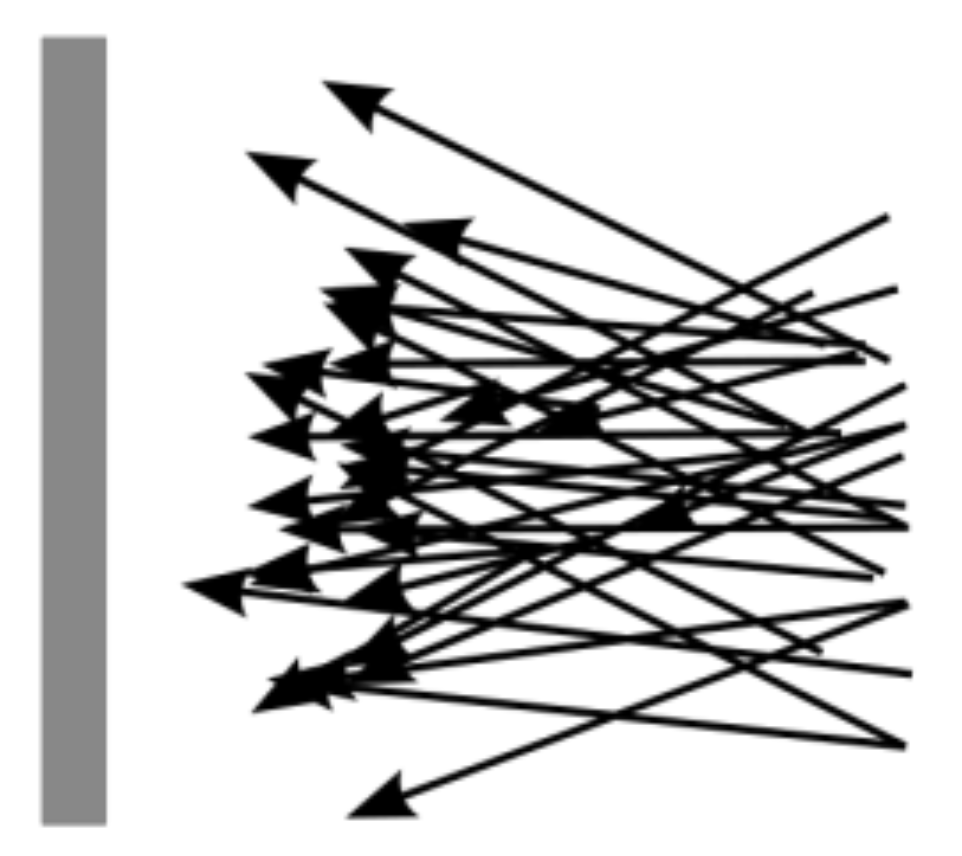
\includegraphics[width=0.5\linewidth]{collimatora.png}
            \caption{Before collimation.}
            \label{fig:collimatora}
        \end{subfigure}
        \begin{subfigure}[b]{0.3\linewidth}
            \centering
            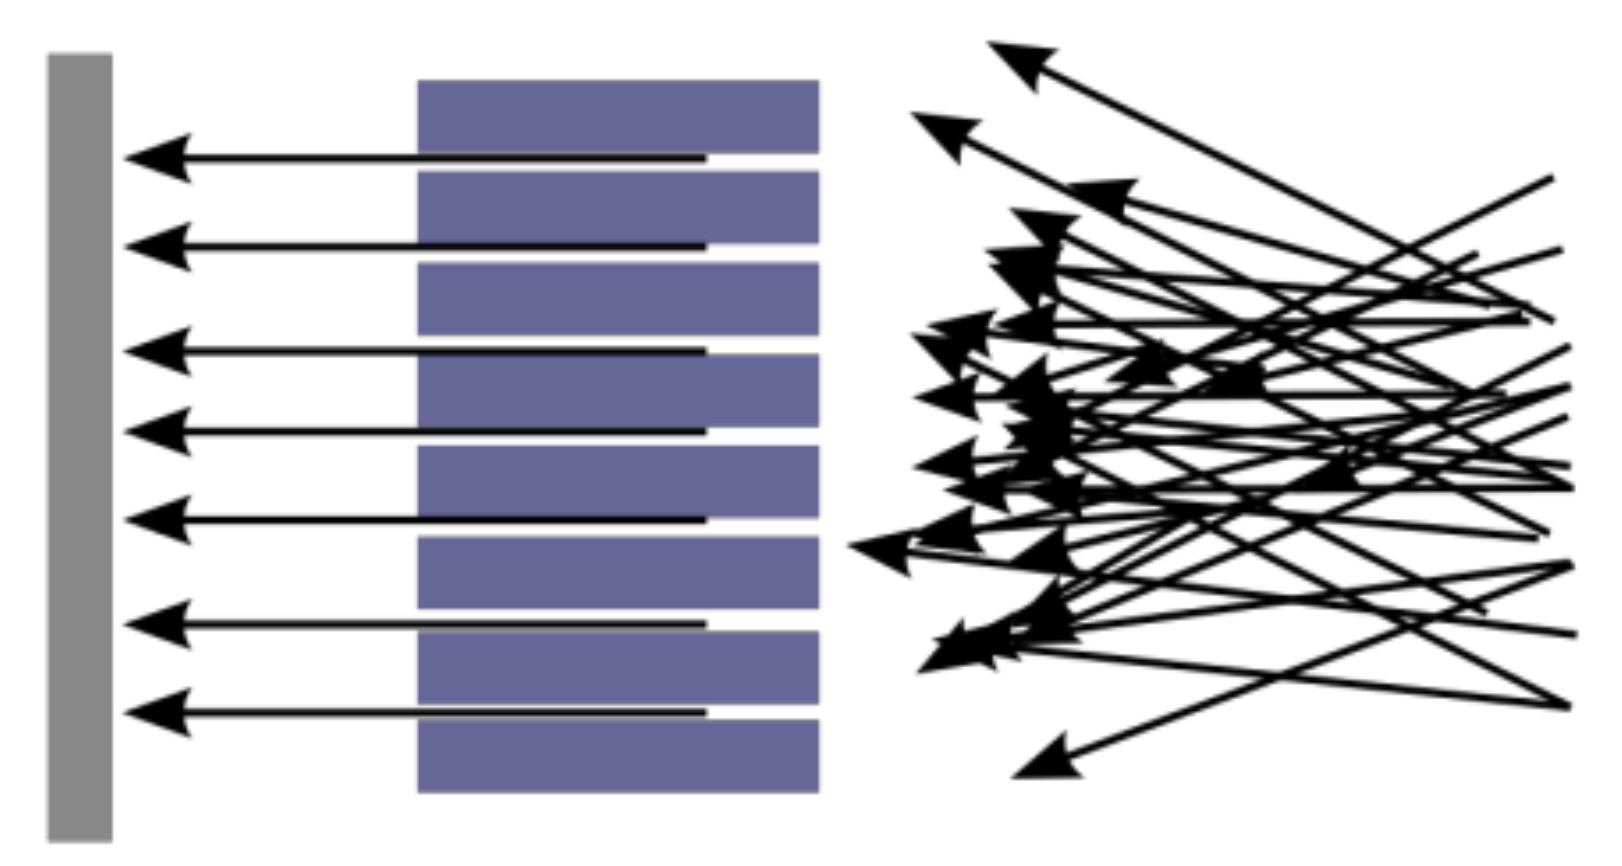
\includegraphics[width=0.8\linewidth]{collimatorb.png}
            \caption{After collimation.}
            \label{fig:collimatorb}
        \end{subfigure}
        \caption{Collimator function.}
        \label{fig:collimator}
    \end{figure}
    \begin{itemize}
        \item A generated X-ray beam is far from perfect; the X-rays go in many directions.
        \item Solution: Use a collimator.
        \item Typically lead, but can be tungsten, molybdenum, tin, bismuth, high density plastics, etc.
        \begin{itemize}
            \item Lead is preferred because of its high density and low cost.
        \end{itemize}
        \item Mechanism: Most X-rays get absorbed; the right ones (straight forward ones) pass through.
    \end{itemize}
    \item How a diffractometer is made.
    \begin{figure}[h!]
        \centering
        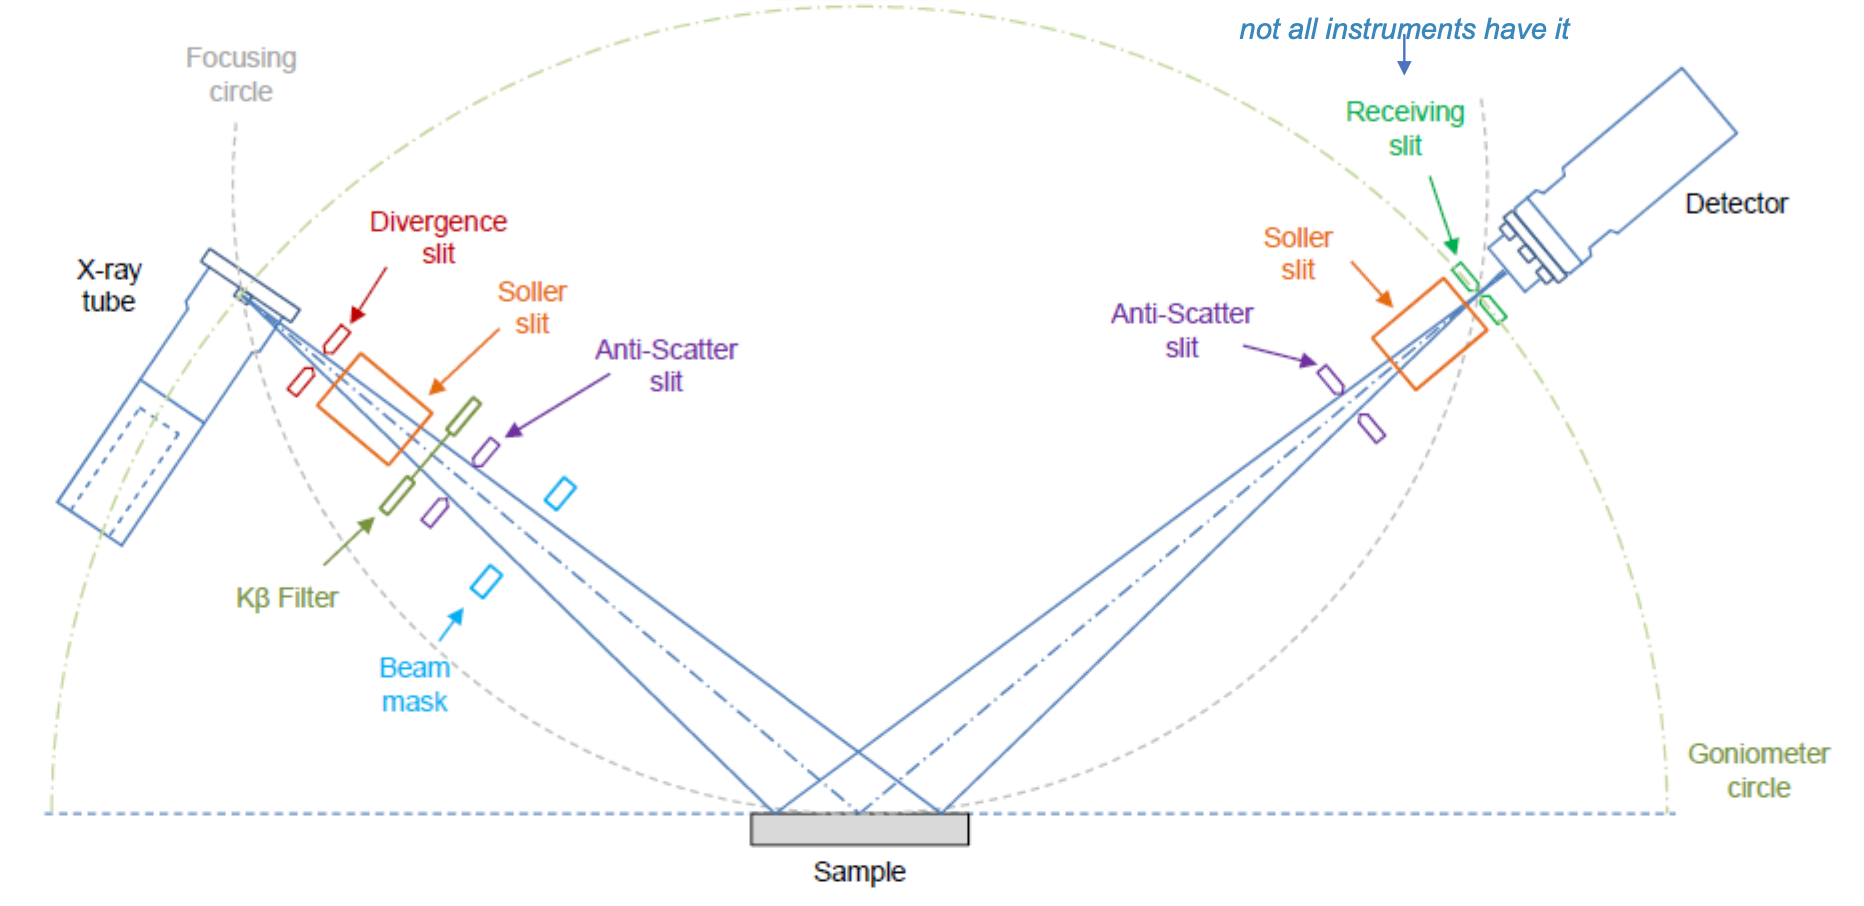
\includegraphics[width=0.9\linewidth]{diffractometerConfiguration.png}
        \caption{Typical diffractometer configuration.}
        \label{fig:diffractometerConfiguration}
    \end{figure}
    \begin{itemize}
        \item X-rays are generated and emitted by an X-ray source.
        \item Next, they pass through a \textbf{divergence slit}, which limits the total irradiation area of the sample.
        \begin{itemize}
            \item At higher $2\theta$ angles, less area is irradiated, which decreases diffraction intensity. The depth of penetration of the beam becomes commensurably deeper with higher angles.
        \end{itemize}
        \item Then its into the sample chamber.
        \item After that, they pass through \textbf{scatter slits}, which address the scattering because of "too thick" samples, rough samples, scattering from the substrate or material matrix, etc.
        \item Another round of slits is the \textbf{Soller slits}.
        \item The final "filter" is a monochromator, which removes 75\% of the unwanted wavelengths.
        \item Finally, the X-rays arrive at the detector.
    \end{itemize}
    \item There is another diffractometer schematic and a labeled picture of an actual one in the slides.
    \item Examples of slits and masks.
    \begin{itemize}
        \item \textbf{Divergence slits}, \textbf{beam masks}, \textbf{programmable divergence slits}, and Soller slits.
    \end{itemize}
    \item \textbf{Divergence slit}: A piece of metal with an opening of a certain width.
    \item Fixed vs. variable divergence slits.
    \begin{figure}[h!]
        \centering
        \begin{subfigure}[b]{\linewidth}
            \centering
            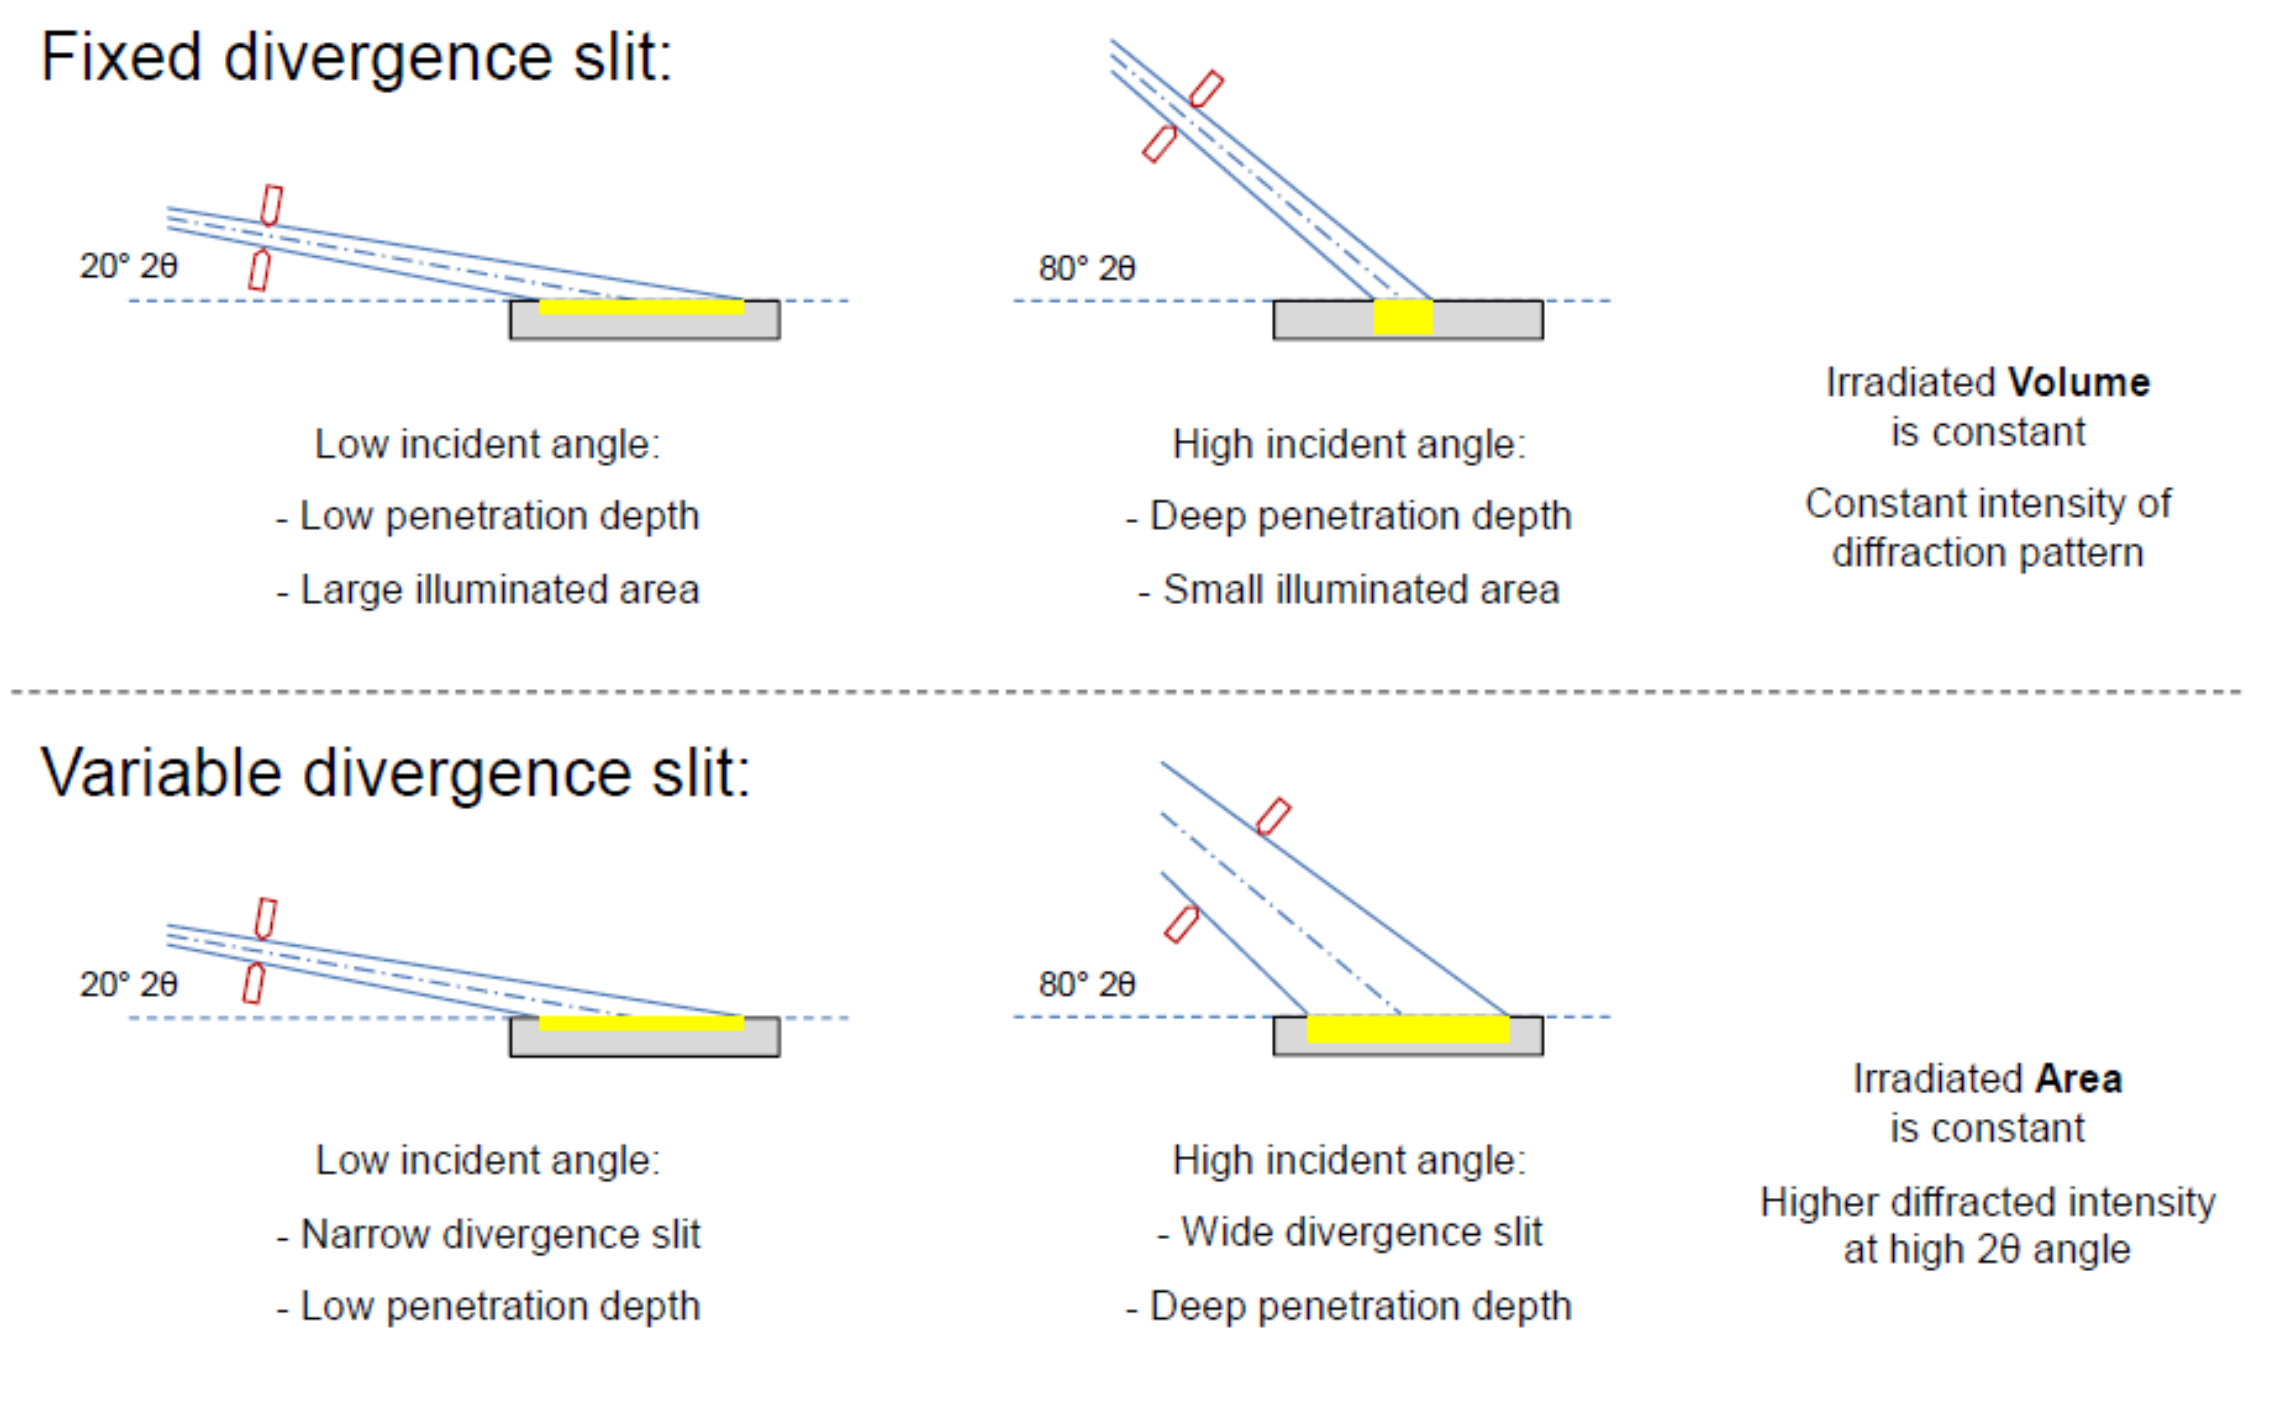
\includegraphics[width=0.7\linewidth]{fixedVsVariablea.png}
            \caption{Angle of incidence.}
            \label{fig:fixedVsVariablea}
        \end{subfigure}\\[2em]
        \begin{subfigure}[b]{\linewidth}
            \centering
            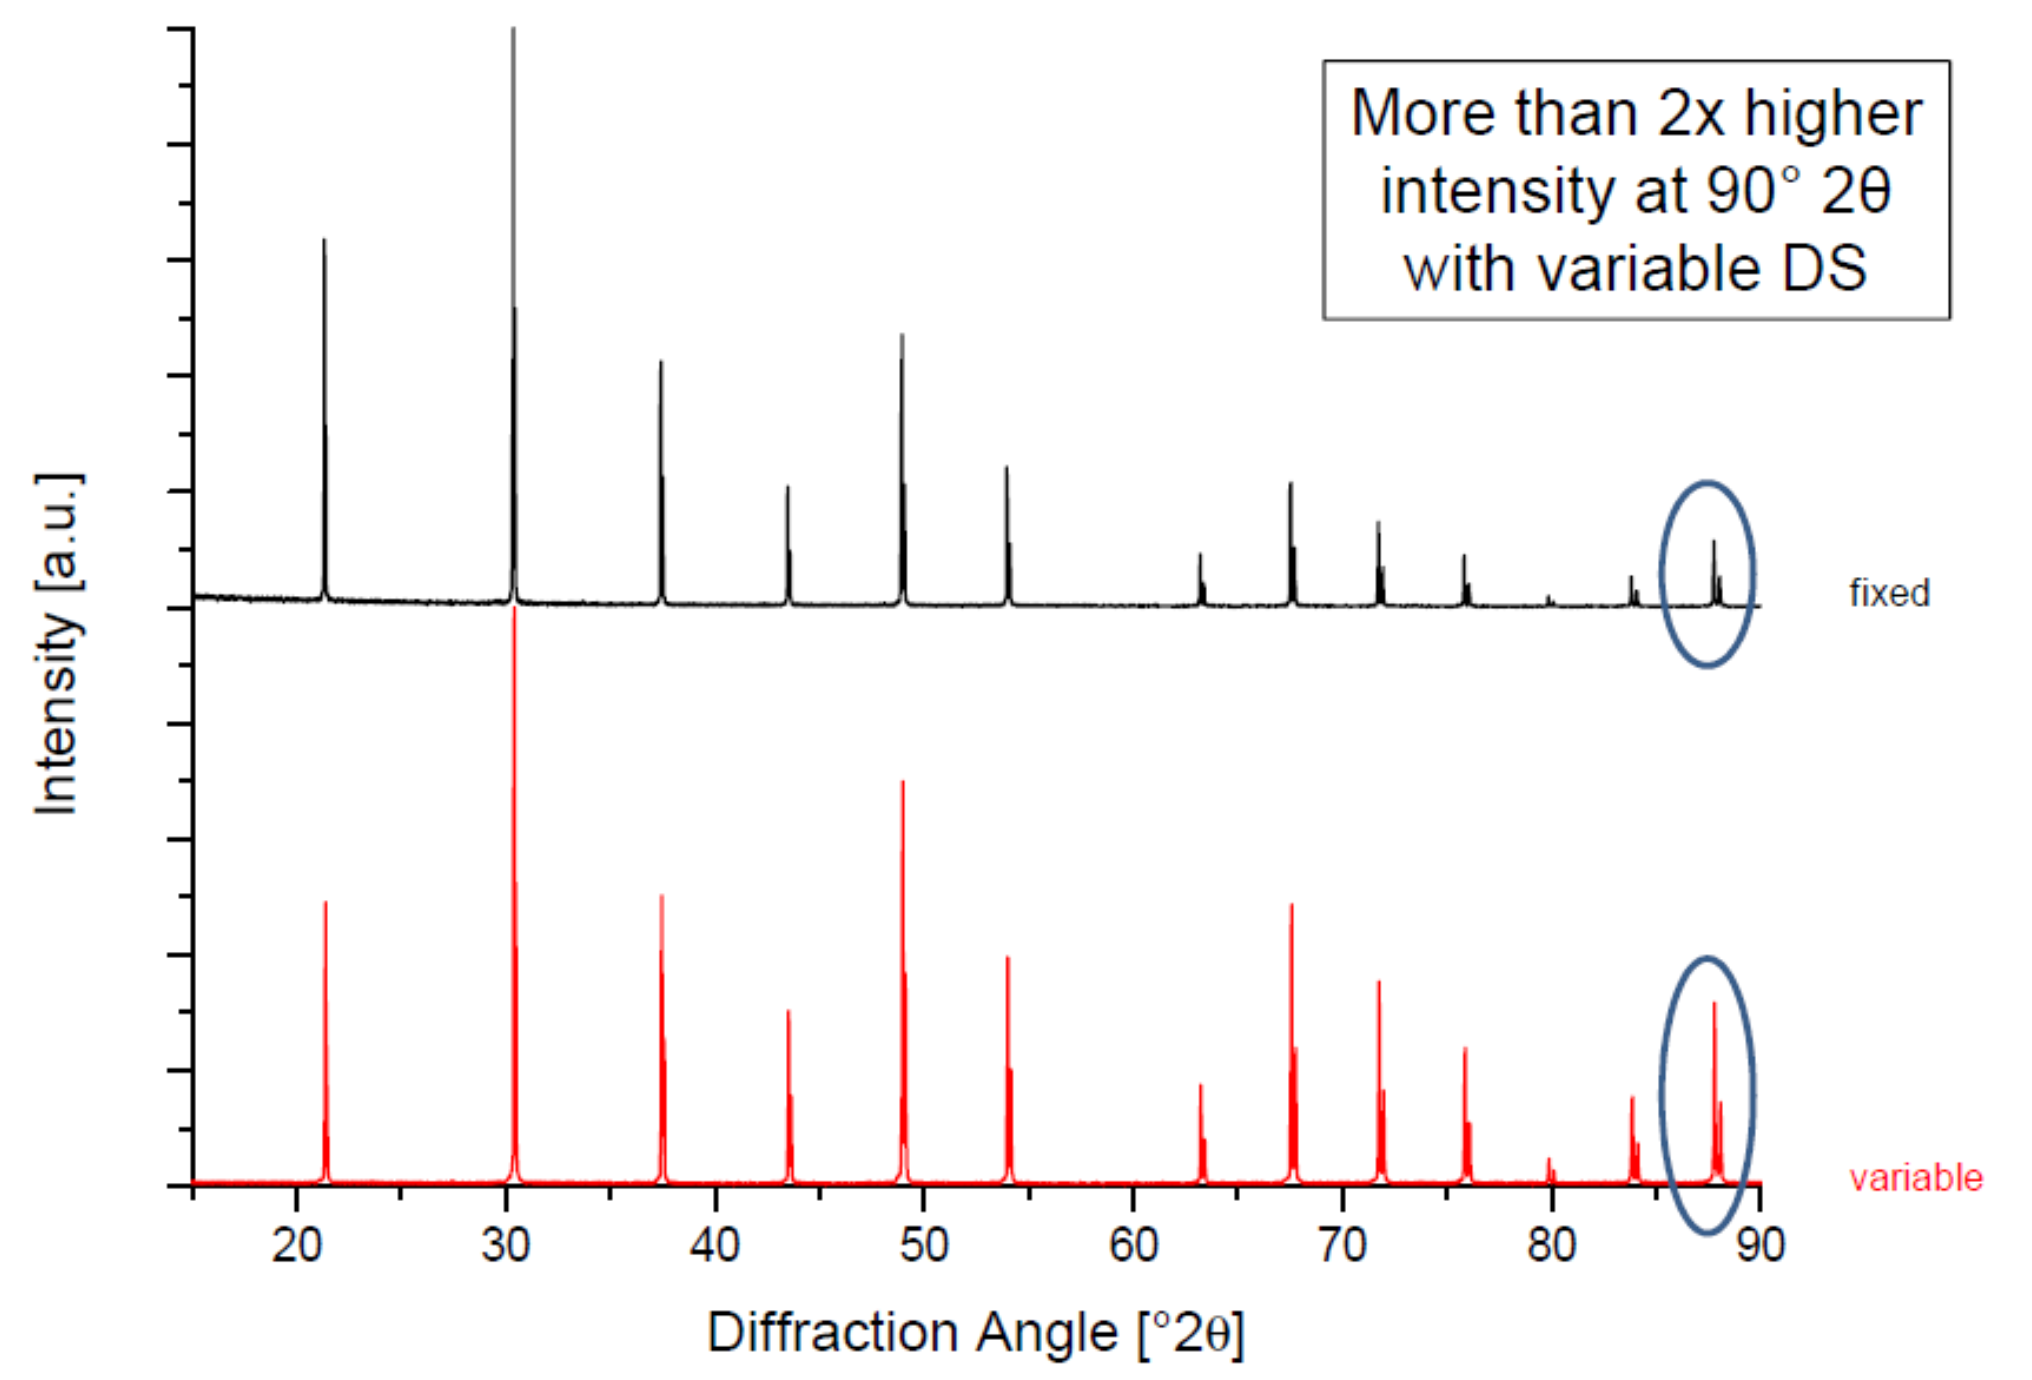
\includegraphics[width=0.5\linewidth]{fixedVsVariableb.png}
            \caption{Spectrum.}
            \label{fig:fixedVsVariableb}
        \end{subfigure}
        \caption{Fixed vs. variable divergence slits.}
        \label{fig:fixedVsVariable}
    \end{figure}
    \begin{itemize}
        \item Fixed divergence slit: As the angle changes, the amount of surface area illuminated decreases.
        \item With a variable divergence slit, we can solve this issue.
        \item Signals are the same at low $2\theta$; signals differ in intensity at high $2\theta$.
    \end{itemize}
    \item \textbf{Beam mask}: Similar to a divergence slit.
    \item \textbf{Programmable divergence slit}: A divergence slit with slots for a beam mask, Soller slits, and attenuation foil or a $\beta$-filter.
    \item \textbf{Soller slits}: A stack of metal films that enable removal of $\sim 99\%$ of the unwanted wavelengths of radiation from the beam. \emph{Also known as} \textbf{receiving slits}, \textbf{RSm slits}.
    \begin{itemize}
        \item These are a part of the instrument and you cannot touch them.
        \item Not all instruments have these.
    \end{itemize}
    \item Most commmon targets for X-ray tubes.
    \begin{itemize}
        \item Usually copper, especially for crystallography.
        \item Medical X-ray tubes use tungsten.
        \item Softer X-rays are needed for mammography, so molybdenum is used.
    \end{itemize}
    \item Detectors.
    \begin{itemize}
        \item For lab experiments, the characteristic emission lines of metal targets such as \ce{Cr}, \ce{Cu}, \ce{Co}, and \ce{Mo} are used in X-ray tubes.
        \item Therefore, the detector should detect X-ray photons with energies in the range of \SIrange{5}{20}{\kilo\electronvolt}. The background bremsstrahlung photons (an unwanted byproduct) have energies up to \SI{55}{\kilo\electronvolt}.
        \item There are two types of detectors.
        \begin{enumerate}[label={(\roman*)}]
            \item \textbf{Photon counting} detectors.
            \item \textbf{Integrating} detectors.
        \end{enumerate}
    \end{itemize}
    \item \textbf{Photon counting} (detector): A detector that, during a measurement, converts the energy of each individual photon into a charge and registers the charge package. \emph{Also known as} \textbf{digital}.
    \item \textbf{Integrating} (detector): A detector that integrates (or "adds up") the charge that is generated due to the conversion of the photon's energy into electric charge. \emph{Also known as} \textbf{analog}.
    \begin{itemize}
        \item The energy information of the photons that are detected is lost and cannot be recovered.
    \end{itemize}
    \item Types of the detectors.
    \begin{itemize}
        \item \textbf{Point}, \textbf{linear}, and \textbf{area} detectors.
        \item These are 0D, 1D, and 2D, respectively.
        \item What are these??
        \item Typical brands listed.
    \end{itemize}
    \item \textbf{Point} (detector): A detector in which the receiving slit determines the active height.
    \item \textbf{Linear} (detector): A detector comprised of a linear array of solid state detectors.
    \item \textbf{Area} (detector): A detector comprised of a 2D array of solid state detectors.
    \item What regimes are used in different instruments?
    \begin{itemize}
        \item Powder sample?
        \begin{itemize}
            \item The scanner moves along a line.
        \end{itemize}
        \item Other important takeaways here??
    \end{itemize}
    \item Examples of detectors.
    \begin{itemize}
        \item Bruker uses a 1D detector and a \ce{Ni} filter.
        \item Certain Panalytical machines also use a 1D detector and a \ce{Ni} filter.
        \item Another type of Panalytical machine uses a 0D detector and a graphite filter.
        \item We can't change the detectors.
    \end{itemize}
    \item Bragg-Brentano geometry.
    \begin{figure}[H]
        \centering
        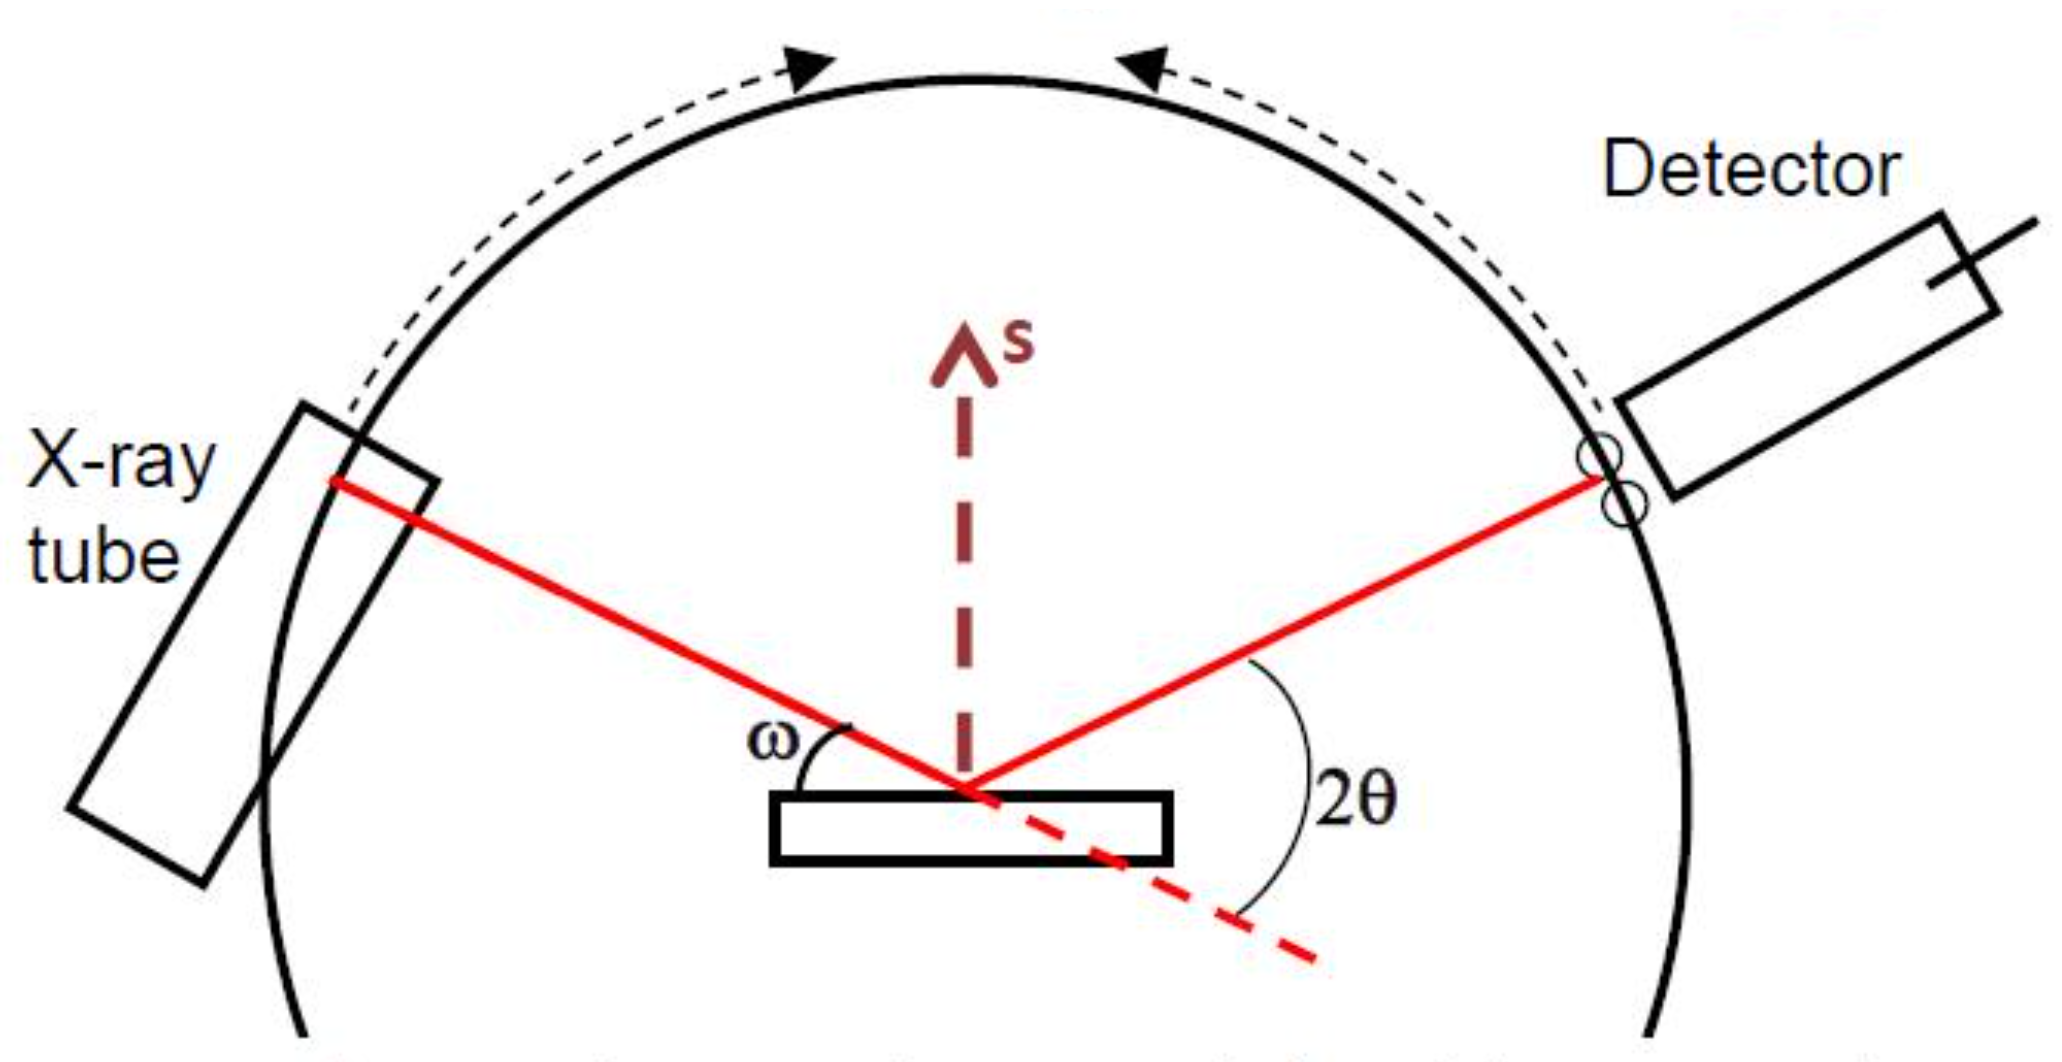
\includegraphics[width=0.4\linewidth]{BraggBrentano.png}
        \caption{Bragg-Brentano geometry.}
        \label{fig:BraggBrentano}
    \end{figure}
    \begin{itemize}
        \item Many diffractometers use this parafocusing geometry.
        \begin{itemize}
            \item Most common; can be used in all types of analysis.
            \item Efficiency is not that great for thin films, though.
        \end{itemize}
        \item The incident- and diffracted-beam slits move on a circle that is centered at the sample. X-rays from the source hit the sample at different points on its surface. During the diffraction process, the X-rays are refocused on the detector slit.
        \item The incident angle $\omega$ between X-ray source and the sample is always half of the detector angle $2\theta$.
        \item Two types of setups.
        \begin{enumerate}
            \item Fixed X-ray tube: The sample rotates at $\theta/\text{min}$ and the detector is always at $2\theta/\text{min}$.
            \item Fixed sample: The tube rotates at the same rate as the detector at $\theta/\text{min}$.
        \end{enumerate}
        \item Sample surface is kept on the tangent plane of the \textbf{focusing circle}.
    \end{itemize}
    \item \textbf{Focusing circle}: The circle lying in the unique plane containing the sample, X-ray source, and receiving slit.
    \item Grazing incidence XRD.
    \begin{itemize}
        \item Helps with thin films.
        \item Other takeaways??
    \end{itemize}
    \item The X-ray spectrum.
    \begin{figure}[h!]
        \centering
        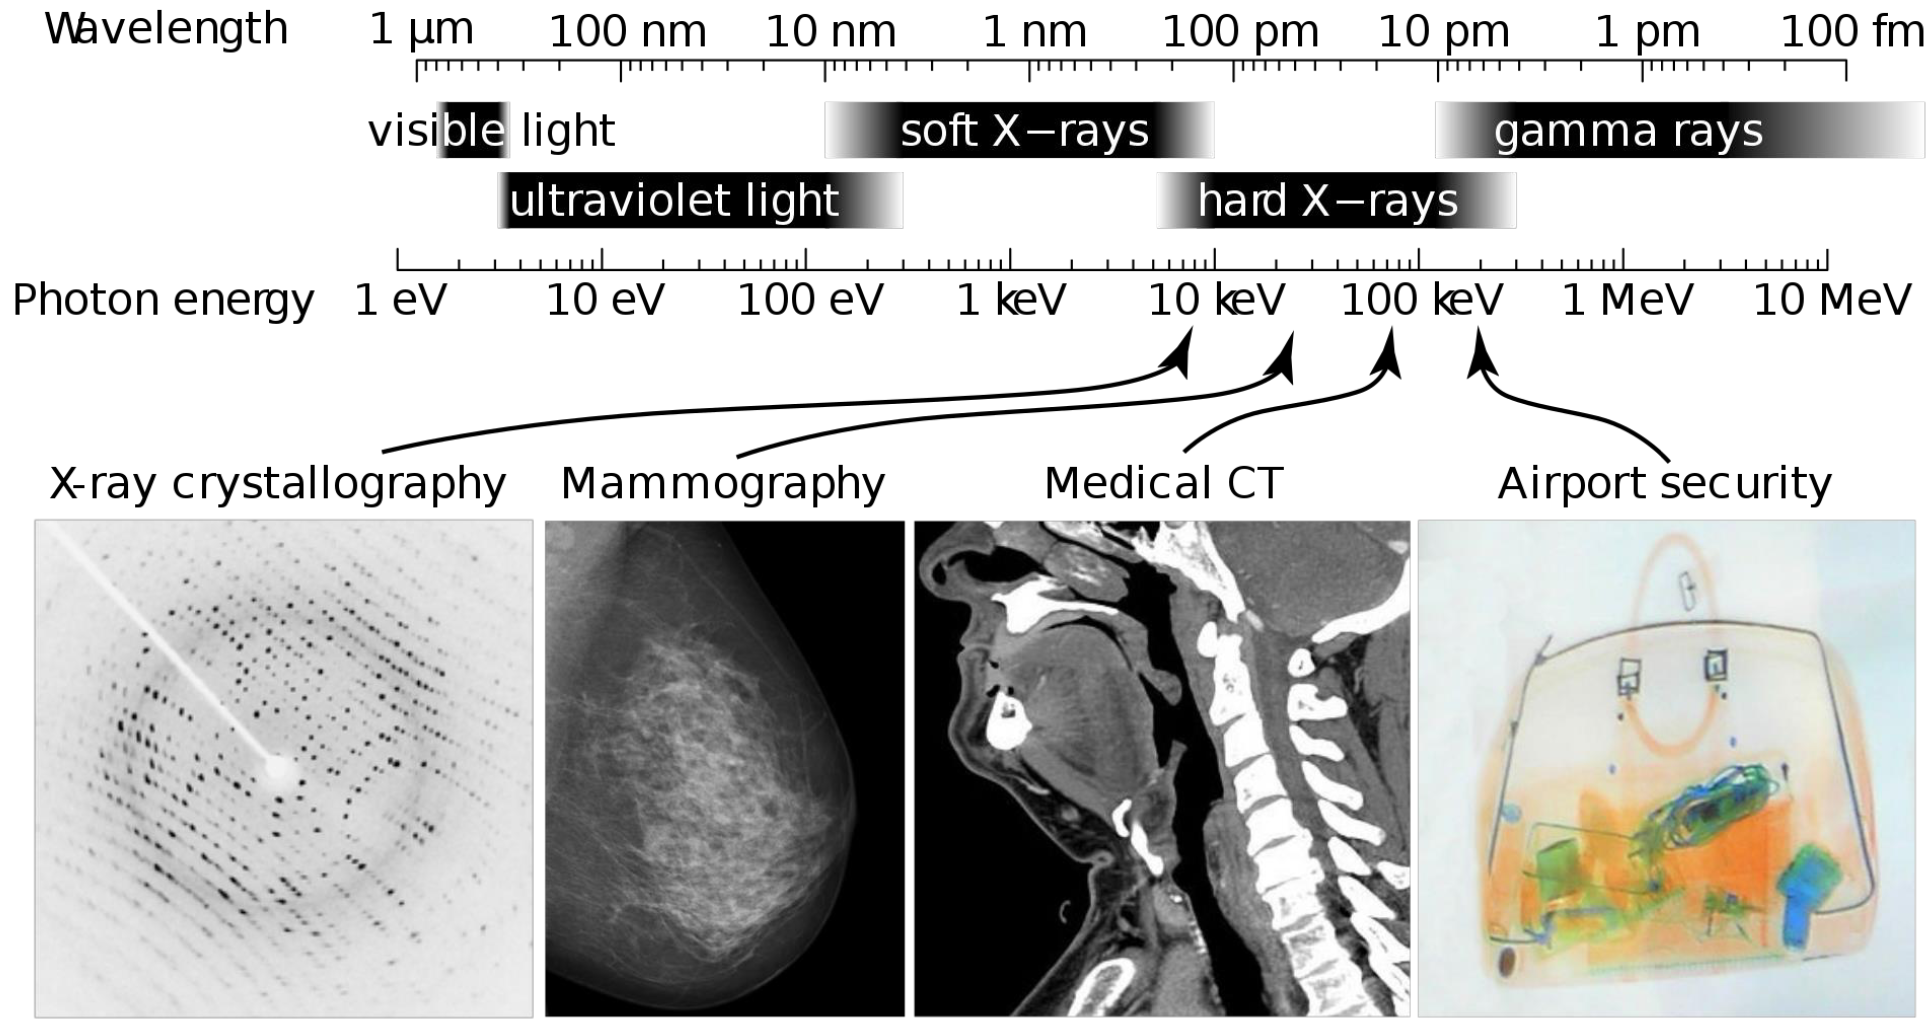
\includegraphics[width=0.65\linewidth]{xraySpectrum.png}
        \caption{X-ray spectrum.}
        \label{fig:xraySpectrum}
    \end{figure}
    \begin{itemize}
        \item Airport (\SI{1000}{\kilo\electronvolt}), medical (\SI{100}{\kilo\electronvolt}), mammography (\SI{10}{\kilo\electronvolt}), X-ray crystallography (\SI{8}{\kilo\electronvolt}).
    \end{itemize}
    \item Applications of X-ray diffraction.
    \begin{itemize}
        \item Same slide as at the beginning.
        \item Shevchenko is really good at circling back to things over and over again so they stick!
    \end{itemize}
    \item Diffraction basics.
    \begin{itemize}
        \item X-rays interact with matter, resulting in \textbf{absorption}, \textbf{elastic scattering}, and \textbf{inelastic scattering}.
    \end{itemize}
    \item \textbf{Absorption}: The energy of the incident photon has to be larger than the \textbf{ionization energy threshold} of an atom or molecule, or the \textbf{work function} of a metal.
    \begin{itemize}
        \item Results in the photoelectric effect, which in turn leads to \textbf{fluorescence}.
        \item Extremely beneficial for elemental analysis.
        \item Absorption is not something we want to see in XRD.
        \begin{itemize}
            \item See earlier discussion of fluorescence.
        \end{itemize}
    \end{itemize}
    \item \textbf{Fluorescence}: The two step process consisting of (1) absorption of radiation by an atom and ionization and (2) relaxation and emission of characteristic radiation.
    \begin{figure}[h!]
        \centering
        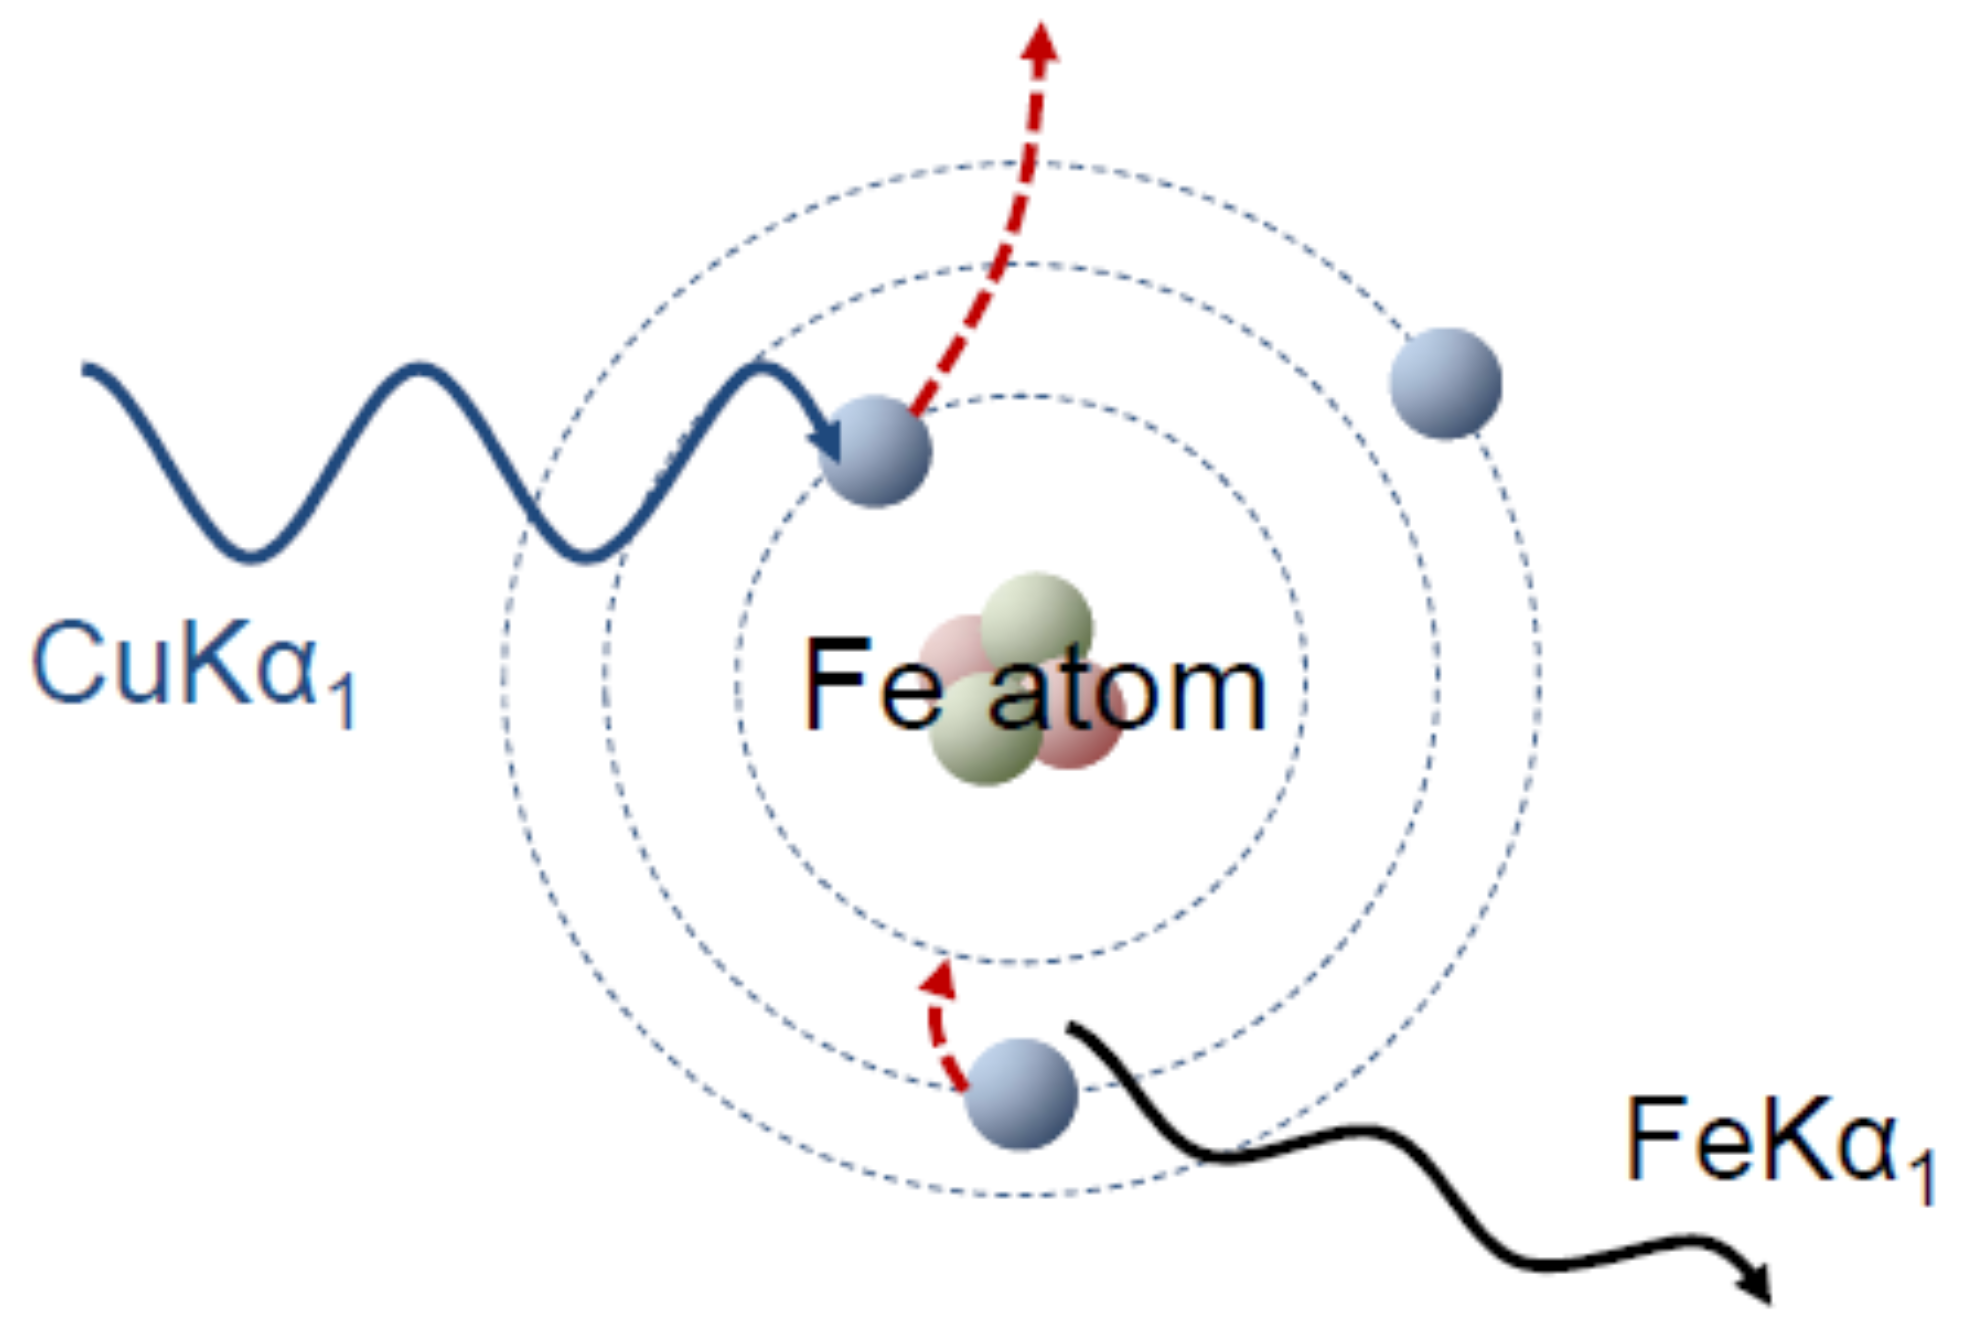
\includegraphics[width=0.3\linewidth]{XRDabsorption.png}
        \caption{Absorption and fluorescence.}
        \label{fig:XRDabsorption}
    \end{figure}
    \item \textbf{Elastic scattering}: Only the \emph{direction} of the scattered photon changes, without changing its initial energy. \emph{Also known as} \textbf{Thomson scattering}.
    \begin{itemize}
        \item The scattering of optical light from electrons was first observed in 1906 by J. J. Thomson.
        \item X-rays are scattered at the electrons of the atomic shell.
        \item X-ray diffraction is a special case of elastic scattering.
    \end{itemize}
    \item \textbf{Inelastic scattering}: The interaction of X-ray photons with a charged particle (electron) resulting in a decrease in energy of the photon. \emph{Also known as} \textbf{Compton scattering}.
    \begin{itemize}
        \item First observed by Arthur Compton in 1923.
        \item The frequency shift has been explained by the momentum transfer of light quanta to the electrons of the material. This provided direct evidence for the quantum nature of light.
        \item Initial energy of the photon is \emph{changing}.
    \end{itemize}
    \item Why X-rays?
    \begin{itemize}
        \item X-ray scattering experiments have played a central role in nearly all areas of physics, chemistry, and material science to study microscopic structure and the state of matter.
        \item We use X-rays because the interatomic distances in crystals are between \SIrange{0.15}{0.4}{\nano\meter} and X-ray wavelengths span this range. Thus, the match is perfect for structure determination.
        \item Indeed, interference phenomena are possible only for features of about $\lambda$.
    \end{itemize}
    \item The first use of X-rays to study crystal structure.
    \begin{itemize}
        \item Reported by Max von Laue (Nobel Prize 1914).
        \item Laue considered crystals in terms of a 3D network of rows of atoms. His analysis is based on the notion that crystals are like 3D diffraction gratings.
        \item Laue utilized white X-radiation (broad spectrum, unfiltered).
        \item The diffraction spots that surrounded the central spot of the primary beam could be explained as an interference pattern due to the crystal's space lattice. Each spot was caused by X-rays that corresponded to a certain lattice constant and wavelength.
    \end{itemize}
    \item Bragg's law.
    \begin{itemize}
        \item Obtained as a result of experiments by William Lawrence Bragg and his father, Sir William Henry Bragg in 1912.
        \item Nobel Prize (1915) for their work determining the crystal structures of \ce{NaCl}, \ce{ZnS}, and diamond, and for "their services in the analysis of crystal structure by means of X-rays."
        \item The Bragg spectrometer had an X-ray tube, filters, collimators, a crystal sample, and a detector.
    \end{itemize}
    \item The principle of Bragg's law.
    \begin{itemize}
        \item We'll start here next class.
    \end{itemize}
    \item Write out ppt. notes ahead of time next time!
\end{itemize}




\end{document}